\documentclass{beamer}
\usetheme{Madrid}
\usecolortheme{whale}

\usepackage{graphicx}
\usepackage{tikz}
\usetikzlibrary{shapes.geometric, arrows.meta, positioning, calc}
\usepackage{booktabs}
\usepackage{listings}
\usepackage{algorithm}
\usepackage{algorithmic}
\usepackage{amsmath}
\usepackage{amssymb}
\usepackage{multirow}
\usepackage{array}

% Define Verilog listing style for presentation
\lstdefinelanguage{Verilog}{
  morekeywords={module, input, output, wire, reg, parameter, localparam, always, assign, begin, end, case, default, endcase, posedge, negedge, if, else, initial},
  sensitive=true,
  morecomment=[l]{//},
  morecomment=[s]{/*}{*/},
  morestring=[b]"
}

\lstset{
  language=Verilog,
  basicstyle=\ttfamily\tiny,
  keywordstyle=\color{blue}\bfseries,
  commentstyle=\color{gray},
  stringstyle=\color{purple},
  backgroundcolor=\color{white},
  showspaces=false,
  showstringspaces=false,
  showtabs=false,
  frame=single,
  tabsize=2,
  breaklines=true,
}

% Custom commands and metadata
\title[Scalable SPI Bus Interface]{Design and FPGA Implementation of a Scalable SPI Bus Interface Supporting Multiple Sensors with Variable Data Widths}
\subtitle{Comprehensive Project Report \& Hardware Verification Presentation}
\author[Bhargav \& Kaushik]{Bhargav Vemparala \\ and \\ Katta Sri Kaushik}
\institute[Evaluation Board]{Department of Electrical and Computer Engineering \\ University Evaluation Board}
\date{August 2026}

\begin{document}

% Slide 1: Title Slide
\begin{frame}
  \titlepage
\end{frame}

% Slide 2: Table of Contents
\begin{frame}{Presentation Outline}
  \tableofcontents
\end{frame}

\section{Introduction \& Evolution}

% Slide 3: Motivation
\begin{frame}{Introduction \& Motivation}
  \begin{itemize}
    \item \textbf{Problem with Traditional SPI:} 
    \begin{itemize}
      \item Standard SPI requires a dedicated Chip Select (CS) line for each slave device.
      \item For $N$ devices, physical wiring complexity is $O(N)$ (requires $N+3$ wires).
      \item Causes PCB routing congestion and depletes GPIO pins on the host MCU.
    \end{itemize}
    \vspace{0.2cm}
    \item \textbf{Proposed Solution:}
    \begin{itemize}
      \item Architect an intelligent \textbf{SPI Bus Interface} on a Xilinx Artix-7 FPGA.
      \item Share a single 3-wire/4-wire bus among all heterogeneous sensors.
      \item Virtualize sensor registers on-chip, reducing wiring complexity to a constant $O(1)$.
    \end{itemize}
    \vspace{0.2cm}
    \item \textbf{Key Innovations:}
    \begin{itemize}
      \item Dual protocol support: \textbf{Address + Bit-Length} (Dynamic) vs. \textbf{ROM Lookup Table} (Static).
      \item Integrated Clock Domain Crossing (CDC) asynchronous FIFO.
      \item Full hardware verification via ESP32 Web Interface and Vivado synthesis.
    \end{itemize}
  \end{itemize}
\end{frame}

% Slide 4: Design Evolution
\begin{frame}{Design Evolution Across Three Iterations}
  \begin{columns}
    \begin{column}{0.33\textwidth}
      \begin{block}{\small Iteration 1: PoC}
        \scriptsize
        \textbf{Single Slave Direct}
        \begin{itemize}
          \item Point-to-point interface.
          \item Fixed 1-bit input/output.
          \item 5-state machine.
          \item High protocol overhead (5 cycles per bit).
        \end{itemize}
      \end{block}
    \end{column}
    \begin{column}{0.33\textwidth}
      \begin{block}{\small Iteration 2: Burst-Mode}
        \scriptsize
        \textbf{Fixed-Width Bus}
        \begin{itemize}
          \item Address decoding added.
          \item Fixed 4-bit burst transfers.
          \item Shared register array.
          \item Inflexible for asymmetric sensors.
        \end{itemize}
      \end{block}
    \end{column}
    \begin{column}{0.33\textwidth}
      \begin{block}{\small Iteration 3: Scalable Architecture}
        \scriptsize
        \textbf{Final Architecture}
        \begin{itemize}
          \item Heterogeneous sensors.
          \item Asymmetric read/write widths.
          \item Dynamic \& ROM protocols.
          \item Decoupled master/sensor domains.
        \end{itemize}
      \end{block}
    \end{column}
  \end{columns}
\end{frame}

\section{System Architecture}

% Slide 5: System Architecture Diagram
\begin{frame}{Generalized System Block Diagram}
  \centering
  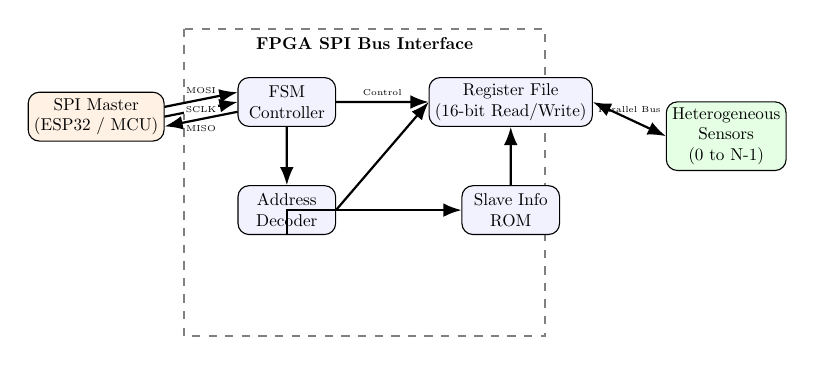
\begin{tikzpicture}[
      scale=0.62, every node/.style={transform shape},
      node distance=1.2cm and 1.5cm,
      block/.style={draw, rectangle, minimum height=1.0cm, minimum width=2.0cm, align=center, fill=blue!5, rounded corners},
      line/.style={draw, -{Latex[scale=1.0]}, thick},
      doubleline/.style={draw, {Latex[scale=1.0]}-{Latex[scale=1.0]}, thick}
  ]
      % Draw Master Block
      \node [block, fill=orange!10] (master) {SPI Master\\(ESP32 / MCU)};
      
      % Draw Bus Interface Boundary (FPGA)
      \draw[dashed, color=gray, thick] (1.8, 1.8) rectangle (9.2, -4.5);
      \node at (5.5, 1.5) {\textbf{FPGA SPI Bus Interface}};

      % Draw Internal Components
      \node [block, right=of master, yshift=0.3cm] (fsm) {FSM\\Controller};
      \node [block, below=of fsm] (decoder) {Address\\Decoder};
      \node [block, right=of fsm, xshift=0.4cm] (regs) {Register File\\(16-bit Read/Write)};
      \node [block, below=of regs] (rom) {Slave Info\\ROM};
      
      % Draw Sensors Block
      \node [block, right=of regs, fill=green!10, yshift=-0.7cm] (sensors) {Heterogeneous\\Sensors\\(0 to N-1)};
      
      % Connect Master to Interface
      \path [line] ($(master.east)+(0,0.2)$) -- node[above, font=\tiny] {MOSI} ($(fsm.west)+(0,0.2)$);
      \path [line] ($(fsm.west)+(0,-0.2)$) -- node[below, font=\tiny] {MISO} ($(master.east)+(0,-0.2)$);
      \path [line] (master.east) -- node[fill=white, inner sep=1pt, font=\tiny] {SCLK} (fsm.west);
      
      % Connect internal modules
      \path [line] (fsm.south) -- (decoder.north);
      \path [line] (decoder.east) -- (regs.west);
      \path [line] (decoder.south) |- (rom.west);
      \path [line] (rom.north) -- (regs.south);
      \path [line] (fsm.east) -- node[above, font=\tiny] {Control} (regs.west);
      
      % Connect Interface to Sensors
      \path [doubleline] (regs.east) -- node[above, font=\tiny] {Parallel Bus} (sensors.west);
  \end{tikzpicture}
\end{frame}

% Slide 6: Core Submodules
\begin{frame}{Core FPGA Internal Submodules}
  \begin{itemize}
    \item \textbf{FSM Controller:} Coordinates incoming serial streams on MOSI, decodes command opcodes, and drives serial bit shifting.
    \item \textbf{Address Decoder:} Maps incoming address frames directly to target virtual sensor register slices.
    \item \textbf{Register File:} 16-bit split register space:
    \begin{itemize}
      \item \texttt{read\_reg} (16-bit): Captures live parallel sensor readings.
      \item \texttt{write\_reg} (16-bit): Stores master control outputs.
    \end{itemize}
    \item \textbf{Snapshot Controller:} Latches sensor register values into shadow registers at the start of read transactions to prevent data tearing during multi-bit transfers.
  \end{itemize}
\end{frame}

% Slide 7: Clock Domain Crossing (CDC)
\begin{frame}{Clock Domain Crossing \& FIFO Synchronization}
  \begin{itemize}
    \item \textbf{Asynchronous Domain Challenge:} Sensors operate on $\text{CLK}_{\text{sensor}}$ while the SPI host communicates on an independent, bursty $\text{SCLK}$.
    \item \textbf{Metastability Mitigation:} 
    \begin{itemize}
      \item Direct cross-domain sampling leads to timing violations and glitches.
      \item Integrated a 16-bit wide, depth-8 \textbf{Asynchronous CDC FIFO} buffer.
      \item Write port driven by $\text{CLK}_{\text{sensor}}$; read port driven by $\text{SCLK}$.
      \item Dual-rank Gray-code synchronizers protect read/write pointer boundaries.
    \end{itemize}
  \end{itemize}
\end{frame}

\section{Implemented Methodologies}

% Slide 8: Method 1: Address + Length Protocol
\begin{frame}{Method 1: Address + Bit-Length Protocol}
  \begin{itemize}
    \item \textbf{Dynamic Packet Concept:} Master explicitly specifies transaction payload size on the fly for write operations.
    \item \textbf{Packet Breakdown:}
    \begin{itemize}
      \item \textbf{Mode (2 bits):} \texttt{00}=Read, \texttt{01}=Write, \texttt{10}=Reset, \texttt{11}=WHOAMI.
      \item \textbf{Address (5 bits):} Target base offset ($A_4 \dots A_0$).
      \item \textbf{Length (4 bits):} Transmitted in writes; defines payload bit count minus 1.
    \end{itemize}
    \item \textbf{Master-Terminated Reads:} Reads omit the length field. Master keeps MOSI=1 to continue reading, pulls MOSI=0 to terminate.
  \end{itemize}
  \begin{table}
    \centering\tiny
    \begin{tabular}{lcccc}
      \toprule
      \textbf{Op} & \textbf{Mode (2b)} & \textbf{Address (5b)} & \textbf{Length (4b)} & \textbf{Data Payload} \\
      \midrule
      Read & \texttt{00} & $A_4 \dots A_0$ & N/A & Dynamic (MOSI=0 to stop) \\
      Write & \texttt{01} & $A_4 \dots A_0$ & $L_3 \dots L_0$ & Variable ($L+1$ bits) \\
      \bottomrule
    \end{tabular}
  \end{table}
\end{frame}

% Slide 9: Method 1 FSM & Timing
\begin{frame}{Method 1: FSM State Diagram \& Write Timing}
  \begin{columns}
    \begin{column}{0.5\textwidth}
      \centering
      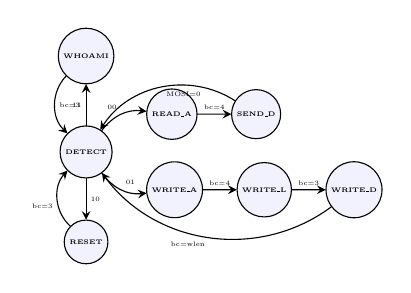
\begin{tikzpicture}[
          scale=0.48, every node/.style={transform shape},
          ->, >=stealth, node distance=1.1cm and 0.9cm,
          state/.style={circle, draw, minimum size=0.9cm, font=\tiny\bfseries, align=center, fill=blue!5},
          transition/.style={font=\tiny, auto}
      ]
          \node[state] (detect) {DETECT};
          \node[state, right=of detect, yshift=1.0cm] (raddr) {READ\_A};
          \node[state, right=of raddr] (rdata) {SEND\_D};
          \node[state, right=of detect, yshift=-1.0cm] (waddr) {WRITE\_A};
          \node[state, right=of waddr] (wlen) {WRITE\_L};
          \node[state, right=of wlen] (wdata) {WRITE\_D};
          \node[state, below=of detect] (srst) {RESET};
          \node[state, above=of detect] (who) {WHOAMI};

          \path (detect) edge[bend left] node[transition] {00} (raddr);
          \path (detect) edge[bend right] node[transition] {01} (waddr);
          \path (detect) edge node[transition] {10} (srst);
          \path (detect) edge node[transition] {11} (who);
          \path (raddr) edge node[transition] {bc=4} (rdata);
          \path (rdata) edge[bend right=45] node[transition] {MOSI=0} (detect);
          \path (waddr) edge node[transition] {bc=4} (wlen);
          \path (wlen) edge node[transition] {bc=3} (wdata);
          \path (wdata) edge[bend left=45] node[transition] {bc=wlen} (detect);
          \path (srst) edge[bend left=45] node[transition] {bc=3} (detect);
          \path (who) edge[bend right=45] node[transition] {bc=3} (detect);
      \end{tikzpicture}
    \end{column}
    \begin{column}{0.5\textwidth}
      \centering
      \resizebox{\linewidth}{!}{%
      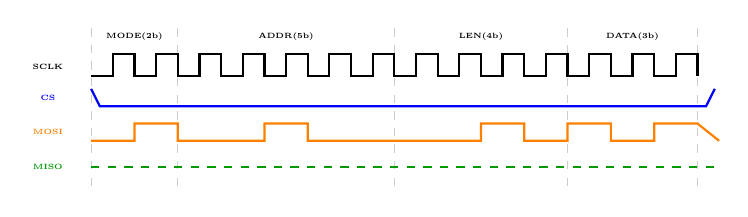
\begin{tikzpicture}[scale=0.55, every node/.style={transform shape}]
          \draw[dashed, gray!40] (0, 1.2) -- (0, -2.5);
          \draw[dashed, gray!40] (2, 1.2) -- (2, -2.5);
          \draw[dashed, gray!40] (7, 1.2) -- (7, -2.5);
          \draw[dashed, gray!40] (11, 1.2) -- (11, -2.5);
          \draw[dashed, gray!40] (14, 1.2) -- (14, -2.5);
          
          \node at (1.0, 1.0) [font=\tiny\bfseries] {MODE(2b)};
          \node at (4.5, 1.0) [font=\tiny\bfseries] {ADDR(5b)};
          \node at (9.0, 1.0) [font=\tiny\bfseries] {LEN(4b)};
          \node at (12.5, 1.0) [font=\tiny\bfseries] {DATA(3b)};

          \node at (-1.0, 0.3) [font=\tiny\bfseries] {SCLK};
          \draw[thick] (0, 0.1) \foreach \x in {1,2,...,14} { -- (\x-0.5, 0.1) -- (\x-0.5, 0.6) -- (\x, 0.6) -- (\x, 0.1) };

          \node at (-1.0, -0.4) [font=\tiny\bfseries, blue] {CS};
          \draw[thick, blue] (0, -0.2) -- (0.2, -0.6) -- (14.2, -0.6) -- (14.4, -0.2);

          \node at (-1.0, -1.2) [font=\tiny\bfseries, orange] {MOSI};
          \draw[thick, orange] (0, -1.4) -- (1, -1.4) -- (1, -1.0) -- (2, -1.0) -- (2, -1.4) -- (4, -1.4) -- (4, -1.0) -- (5, -1.0) -- (5, -1.4) -- (9, -1.4) -- (9, -1.0) -- (10, -1.0) -- (10, -1.4) -- (11, -1.4) -- (11, -1.0) -- (12, -1.0) -- (12, -1.4) -- (13, -1.4) -- (13, -1.0) -- (14, -1.0) -- (14.5, -1.4);

          \node at (-1.0, -2.0) [font=\tiny\bfseries, green!60!black] {MISO};
          \draw[thick, green!60!black, dashed] (0, -2.0) -- (14.5, -2.0);
      \end{tikzpicture}%
      }
      \vspace{0.1cm}
      \tiny Timing diagram for Write 3 bits (\texttt{101}) to address \texttt{0x04}.
    \end{column}
  \end{columns}
\end{frame}

% Slide 10: Method 2: ROM Lookup Table Protocol
\begin{frame}{Method 2: ROM Lookup Table Protocol}
  \begin{itemize}
    \item \textbf{Zero Length Field Overhead:} Sensor register layout metadata is pre-programmed in an on-chip combinational ROM.
    \item \textbf{ROM Table Fields:}
    \begin{itemize}
      \item \texttt{in\_width} / \texttt{out\_width}: Payload bit-widths.
      \item \texttt{in\_start} / \texttt{out\_start}: Starting bit indices within 16-bit register file.
    \end{itemize}
  \end{itemize}
  \begin{table}
    \centering\tiny
    \begin{tabular}{ccccc}
      \toprule
      \textbf{Address (4b)} & \textbf{In Width} & \textbf{Out Width} & \textbf{In Start} & \textbf{Out Start} \\
      \midrule
      \texttt{4'd0} & 3 & 3 & 0 & 0 \\
      \texttt{4'd1} & 3 & 3 & 3 & 3 \\
      \texttt{4'd2} & 3 & 3 & 6 & 6 \\
      \texttt{4'd3} & 3 & 3 & 9 & 9 \\
      \texttt{4'd5} & 4 & 4 & 12 & 12 \\
      \textit{Default} & 1 & 1 & 0 & 0 \\
      \bottomrule
    \end{tabular}
  \end{table}
\end{frame}

% Slide 11: Method 2 FSM & Timing
\begin{frame}{Method 2: FSM Diagram \& Write Timing}
  \begin{columns}
    \begin{column}{0.5\textwidth}
      \centering
      \resizebox{\linewidth}{!}{%
      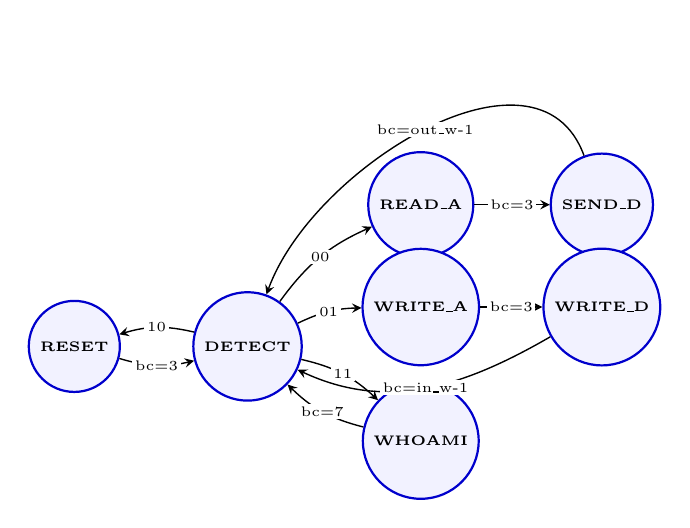
\begin{tikzpicture}[
          ->, >=stealth, line width=0.5pt,
          state/.style={circle, draw=blue!80!black, thick, minimum size=1.0cm, font=\tiny\bfseries, align=center, fill=blue!5},
          transition/.style={font=\tiny, fill=white, inner sep=1pt}
      ]
          \node[state] (detect) at (0, 0) {DETECT};
          \node[state] (raddr) at (2.2, 1.8) {READ\_A};
          \node[state] (rdata) at (4.5, 1.8) {SEND\_D};
          \node[state] (waddr) at (2.2, 0.5) {WRITE\_A};
          \node[state] (wdata) at (4.5, 0.5) {WRITE\_D};
          \node[state] (who) at (2.2, -1.2) {WHOAMI};
          \node[state] (srst) at (-2.2, 0.0) {RESET};

          \path (detect) edge[bend left=15] node[transition] {00} (raddr);
          \path (raddr) edge node[transition] {bc=3} (rdata);
          \path (rdata) edge[out=110, in=70] node[transition] {bc=out\_w-1} (detect);
          \path (detect) edge[bend left=12] node[transition] {01} (waddr);
          \path (waddr) edge node[transition] {bc=3} (wdata);
          \path (wdata) edge[out=210, in=-25] node[transition] {bc=in\_w-1} (detect);
          \path (detect) edge[bend left=15] node[transition] {11} (who);
          \path (who) edge[bend left=15] node[transition] {bc=7} (detect);
          \path (detect) edge[bend right=15] node[transition] {10} (srst);
          \path (srst) edge[bend right=15] node[transition] {bc=3} (detect);
      \end{tikzpicture}%
      }
    \end{column}
    \begin{column}{0.5\textwidth}
      \centering
      \resizebox{\linewidth}{!}{%
      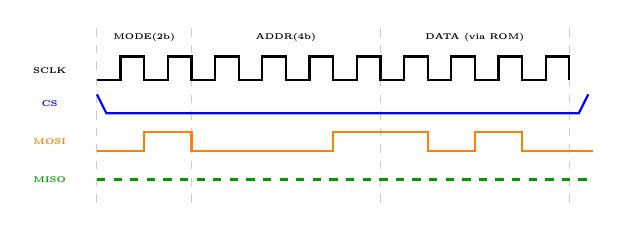
\begin{tikzpicture}[scale=0.6, every node/.style={transform shape}]
          \draw[dashed, gray!40] (0, 1.2) -- (0, -2.5);
          \draw[dashed, gray!40] (2, 1.2) -- (2, -2.5);
          \draw[dashed, gray!40] (6, 1.2) -- (6, -2.5);
          \draw[dashed, gray!40] (10, 1.2) -- (10, -2.5);
          
          \node at (1.0, 1.0) [font=\tiny\bfseries] {MODE(2b)};
          \node at (4.0, 1.0) [font=\tiny\bfseries] {ADDR(4b)};
          \node at (8.0, 1.0) [font=\tiny\bfseries] {DATA (via ROM)};

          \node at (-1.0, 0.3) [font=\tiny\bfseries] {SCLK};
          \draw[thick] (0, 0.1) \foreach \x in {1,2,...,10} { -- (\x-0.5, 0.1) -- (\x-0.5, 0.6) -- (\x, 0.6) -- (\x, 0.1) };

          \node at (-1.0, -0.4) [font=\tiny\bfseries, blue] {CS};
          \draw[thick, blue] (0, -0.2) -- (0.2, -0.6) -- (10.2, -0.6) -- (10.4, -0.2);

          \node at (-1.0, -1.2) [font=\tiny\bfseries, orange] {MOSI};
          \draw[thick, orange] (0, -1.4) -- (1, -1.4) -- (1, -1.0) -- (2, -1.0) -- (2, -1.4) -- (5, -1.4) -- (5, -1.0) -- (7, -1.0) -- (7, -1.4) -- (8, -1.4) -- (8, -1.0) -- (9, -1.0) -- (9, -1.4) -- (10.5, -1.4);

          \node at (-1.0, -2.0) [font=\tiny\bfseries, green!60!black] {MISO};
          \draw[thick, green!60!black, dashed] (0, -2.0) -- (10.5, -2.0);
      \end{tikzpicture}%
      }
      \vspace{0.1cm}
      \tiny Method 2 Write timing (Addr \texttt{4'd1}, 4 payload bits from ROM).
    \end{column}
  \end{columns}
\end{frame}

\section{Verilog Implementation}

% Slide 12: Code Optimizations
\begin{frame}{Verilog Design \& Synthesis Optimizations}
  \begin{itemize}
    \item \textbf{Replacement of Modulo Operators:}
    \begin{itemize}
      \item Modulo operations (\texttt{\% 16}) synthesize to bulky, high-latency division blocks.
      \item Optimized to bitwise AND masks (\texttt{\& 4'b1111}) for instantaneous 1-cycle logic paths.
    \end{itemize}
    \vspace{0.15cm}
    \item \textbf{Single-Driver Assurance:}
    \begin{itemize}
      \item All register array updates strictly contained within a single synchronous posedge block.
      \item Eliminates multi-source driver synthesis conflicts.
    \end{itemize}
    \vspace{0.15cm}
    \item \textbf{Tri-state MISO Buffering:}
    \begin{itemize}
      \item \texttt{assign MiSo = (cs == 1'b0 \&\& mode == 2'b00) ? miso\_reg : 1'bz;}
      \item High-impedance state when \texttt{cs} is inactive guarantees physical line sharing.
    \end{itemize}
  \end{itemize}
\end{frame}

\section{FPGA \& Web Validation}

% Slide 13: Physical FPGA Setup
\begin{frame}{Physical FPGA Testbench Setup}
  \begin{columns}
    \begin{column}{0.5\textwidth}
      \textbf{Hardware Environment:}
      \begin{itemize}
        \item Xilinx Artix-7 FPGA (\texttt{xc7a35tcsg324-1}) synthesized in Vivado.
        \item 16 physical DIP switches emulate live parallel sensor inputs (\texttt{sensor\_data}).
        \item 8-digit multiplexed 7-segment display displays \texttt{read\_reg} and \texttt{write\_reg} in hexadecimal.
        \item Onboard status LEDs monitor CS, SCLK, MISO, MOSI, and FSM mode.
      \end{itemize}
    \end{column}
    \begin{column}{0.5\textwidth}
      \centering
      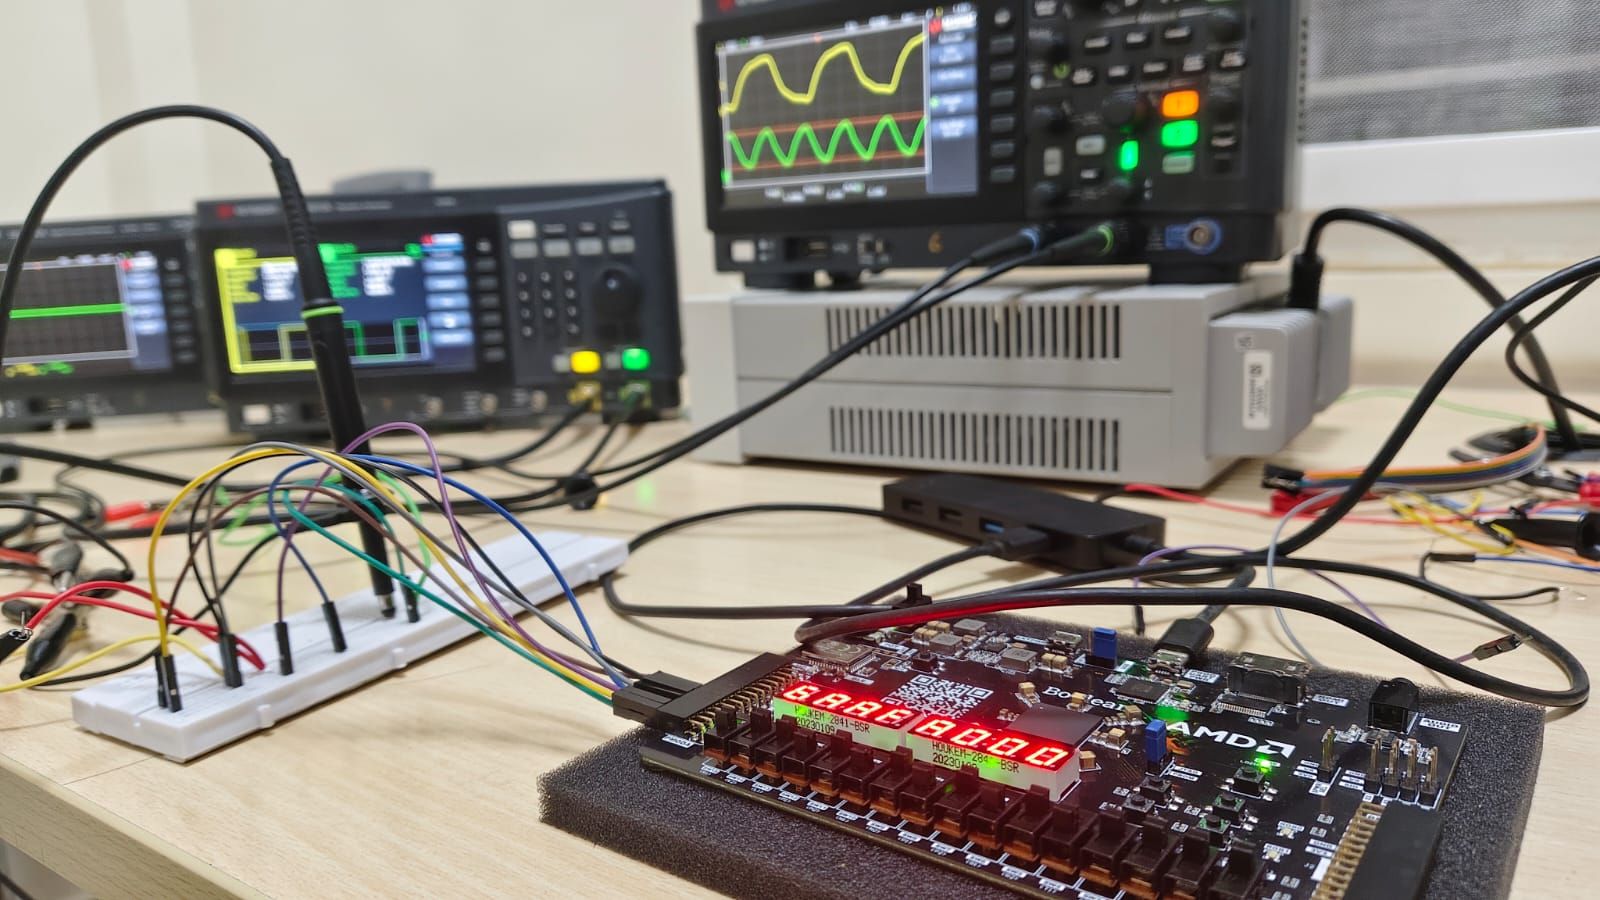
\includegraphics[width=\linewidth]{../images/setup.jpeg}
      \vspace{0.1cm}
      \tiny Physical FPGA Development Board Testbench.
    \end{column}
  \end{columns}
\end{frame}

% Slide 14: FPGA Board Mapping Layout
\begin{frame}{FPGA Top-Level Wrapper Layout (\texttt{fpga\_top.v})}
  \centering
  \resizebox{0.88\linewidth}{!}{%
  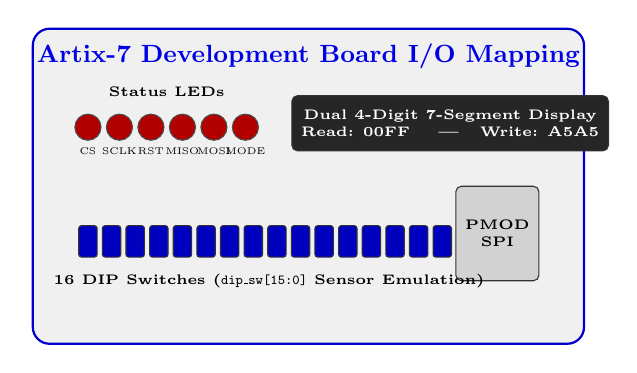
\begin{tikzpicture}[
      board/.style={draw=blue!80!black, fill=gray!12, rounded corners=6pt, thick, minimum height=4.0cm, minimum width=7.0cm},
      component/.style={draw=black!80, rectangle, minimum height=0.7cm, minimum width=2.6cm, fill=black!85, text=white, font=\tiny\bfseries, align=center, rounded corners=2pt},
      led/.style={draw=black!70, circle, minimum size=0.2cm, fill=red!70!black},
      sw/.style={draw=black!80, rectangle, minimum height=0.4cm, minimum width=0.16cm, fill=blue!75!black, rounded corners=1pt},
      pmod/.style={draw=black!80, rectangle, minimum height=1.2cm, minimum width=1.0cm, fill=gray!35, font=\tiny\bfseries, align=center, rounded corners=2pt}
  ]
      \node [board] (pcb) at (0,0) {};
      \node at (0, 1.65) [font=\small\bfseries\color{blue!90!black}] {Artix-7 Development Board I/O Mapping};

      \node at (-1.8, 1.2) [font=\tiny\bfseries] {Status LEDs};
      \foreach \x/\lbl in {-2.8/CS, -2.4/SCLK, -2.0/RST, -1.6/MISO, -1.2/MOSI, -0.8/MODE} {
          \node [led] at (\x, 0.75) {};
          \node at (\x, 0.45) [font=\tiny, scale=0.7] {\lbl};
      }

      \node [component] (seg) at (1.8, 0.8) {Dual 4-Digit 7-Segment Display\\Read: 00FF \quad|\quad Write: A5A5};
      \node [pmod] (pmode) at (2.4, -0.6) {PMOD\\SPI};

      \foreach \x in {-2.8, -2.5, -2.2, -1.9, -1.6, -1.3, -1.0, -0.7, -0.4, -0.1, 0.2, 0.5, 0.8, 1.1, 1.4, 1.7} {
          \node [sw] at (\x, -0.7) {};
      }
      \node at (-0.5, -1.2) [font=\tiny\bfseries] {16 DIP Switches (\texttt{dip\_sw[15:0]} Sensor Emulation)};
  \end{tikzpicture}%
  }
\end{frame}

% Slide 15: ESP32 Integration Flow
\begin{frame}{ESP32 Web Server Integration Topology}
  \begin{itemize}
    \item \textbf{Network Control Architecture:}
    \begin{itemize}
      \item ESP32 microcontroller runs an HTTP / Server-Sent Events (SSE) server.
      \item Provides interactive web controls (Sensor selection, Hex write payload, Read trigger).
      \item ESP32 acts as SPI Master, driving hardware pins on FPGA PMOD headers.
    \end{itemize}
  \end{itemize}
  \vspace{0.2cm}
  \centering
  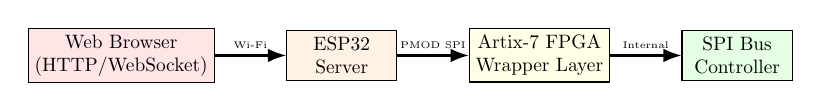
\begin{tikzpicture}[
      scale=0.7, every node/.style={transform shape},
      box/.style={draw, rectangle, minimum height=0.9cm, minimum width=2.0cm, align=center, fill=blue!5},
      arrow/.style={draw, -{Latex[scale=1.0]}, thick}
  ]
      \node [box, fill=red!10] (web) {Web Browser\\(HTTP/WebSocket)};
      \node [box, right=of web, fill=orange!10, xshift=0.3cm] (esp) {ESP32\\Server};
      \node [box, right=of esp, fill=yellow!10, xshift=0.3cm] (fpga) {Artix-7 FPGA\\Wrapper Layer};
      \node [box, right=of fpga, fill=green!10, xshift=0.3cm] (bus) {SPI Bus\\Controller};

      \path [arrow] (web) -- node[above, font=\tiny] {Wi-Fi} (esp);
      \path [arrow] (esp) -- node[above, font=\tiny] {PMOD SPI} (fpga);
      \path [arrow] (fpga) -- node[above, font=\tiny] {Internal} (bus);
  \end{tikzpicture}
\end{frame}

% Slide 16: Web Dashboard Screenshot
\begin{frame}{ESP32 Web Dashboard \& Real-Time Telemetry}
  \centering
  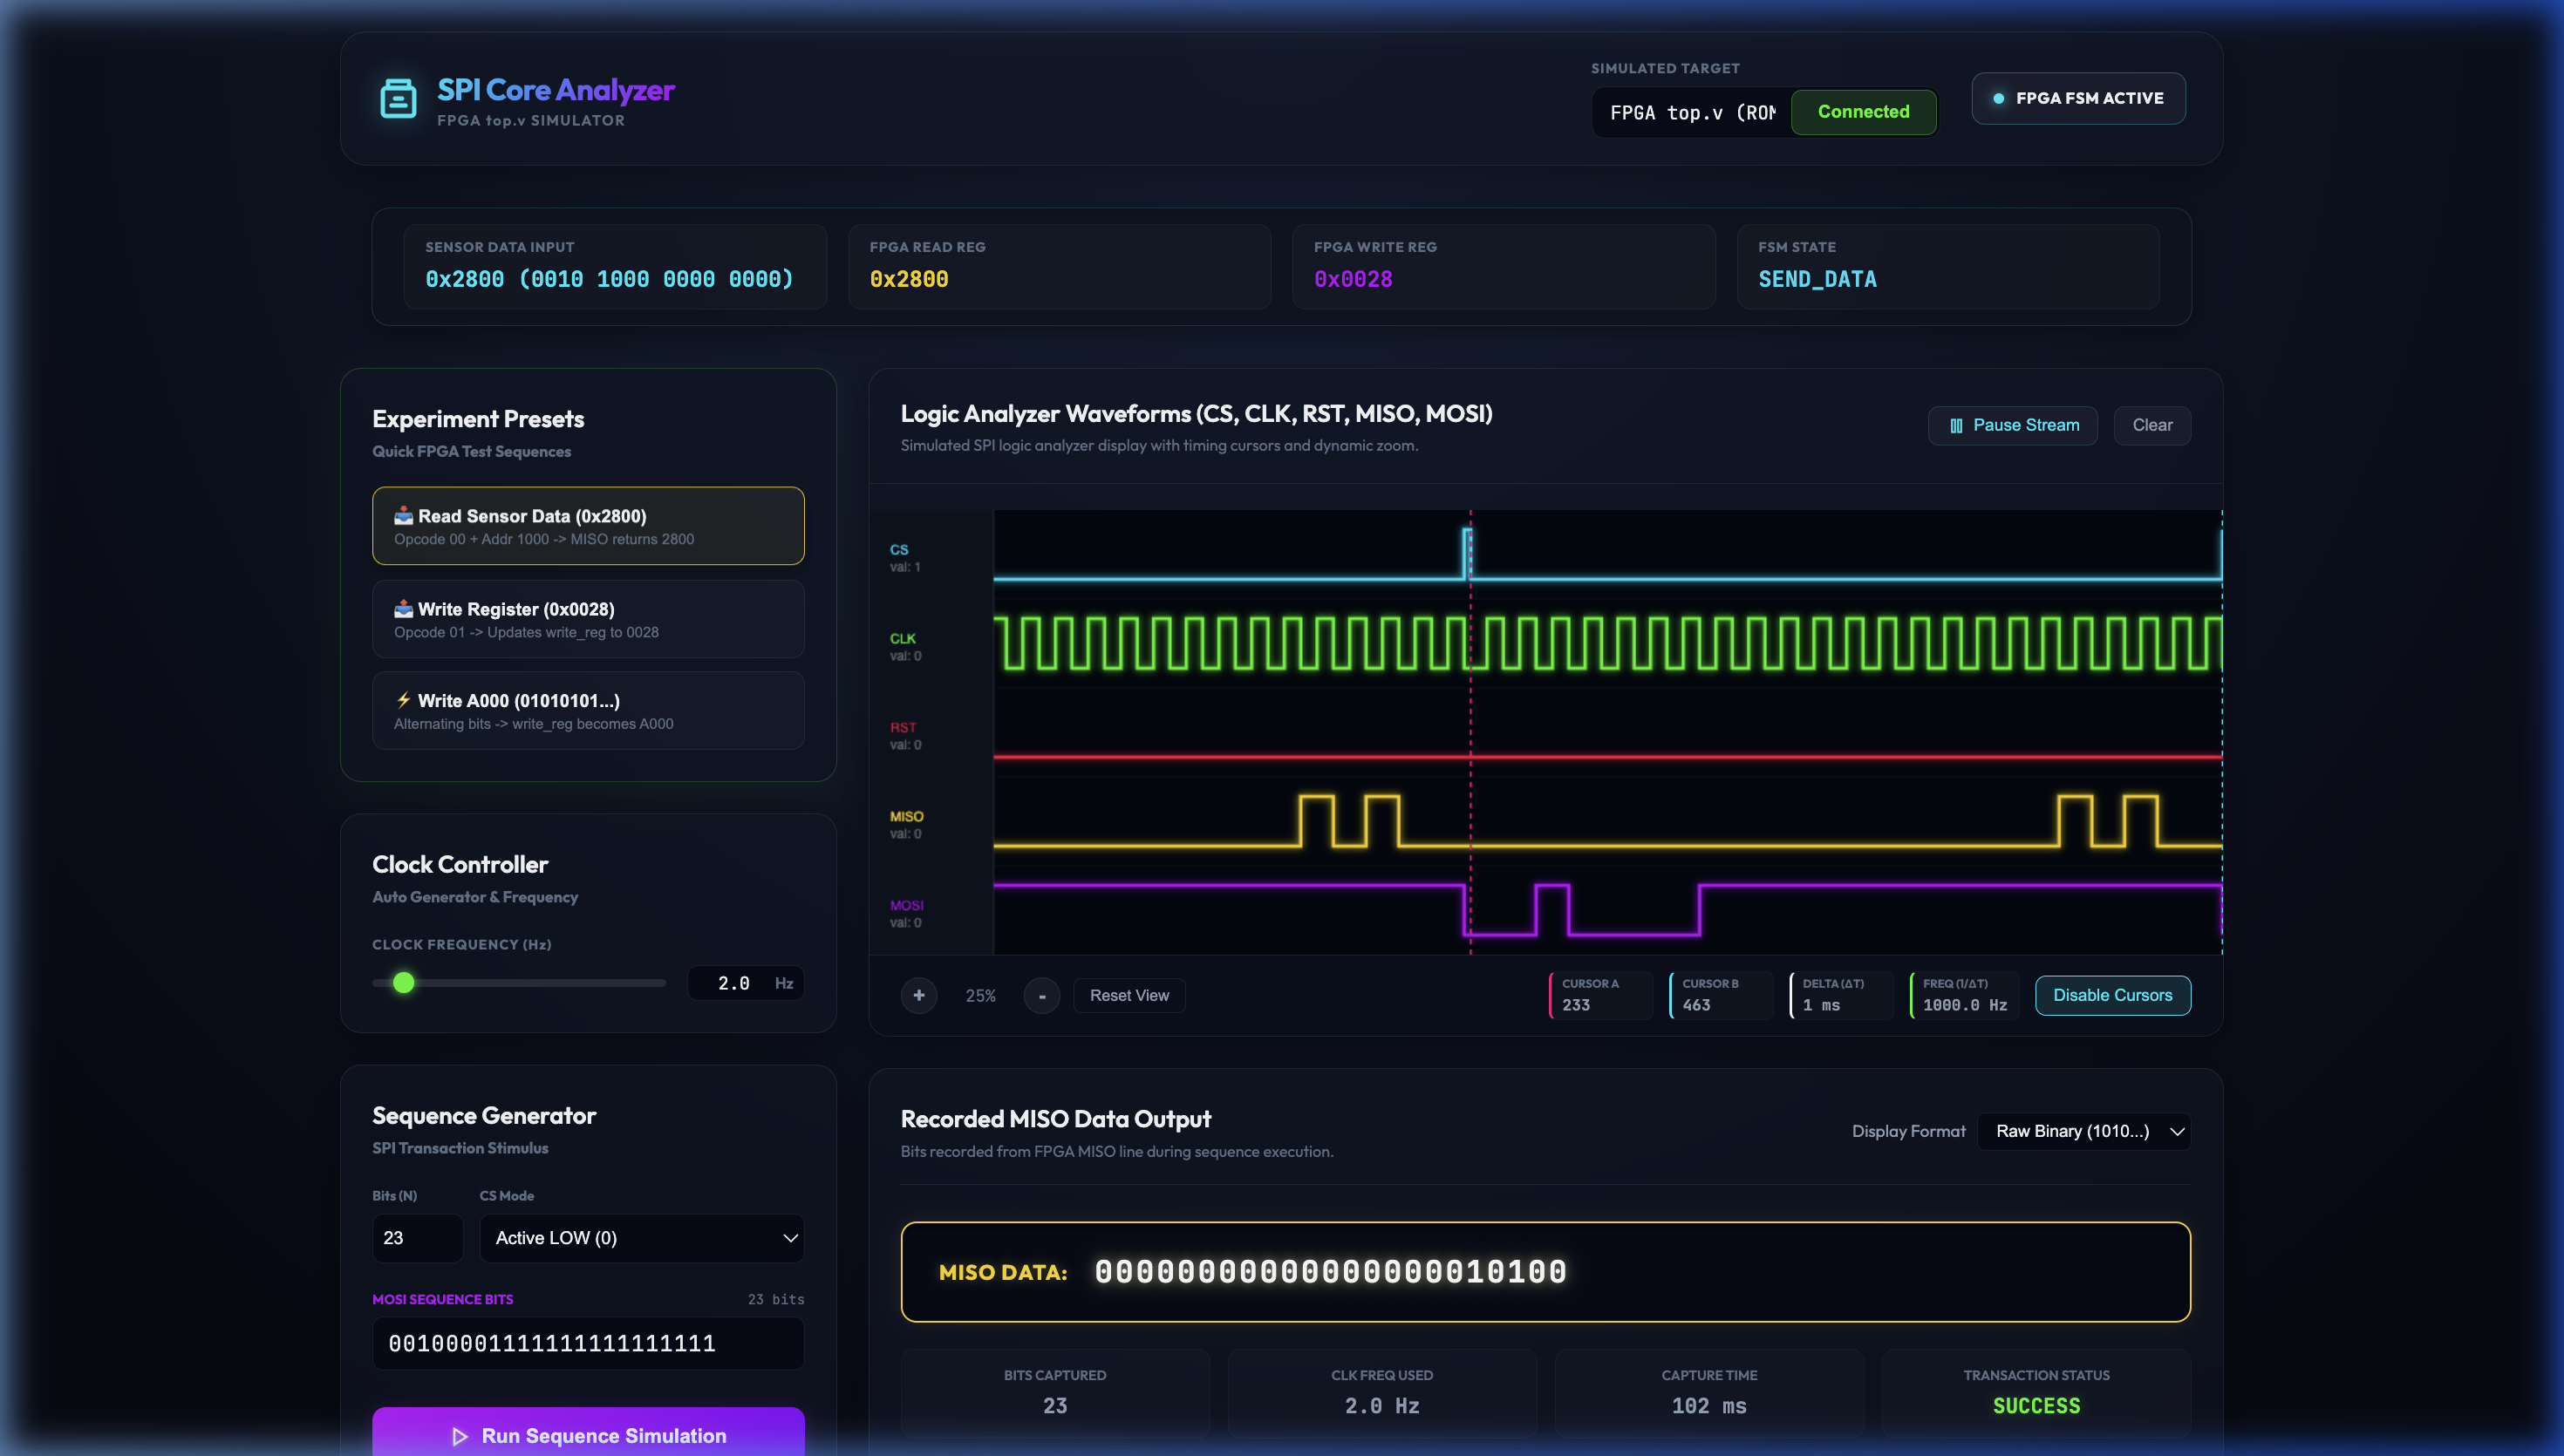
\includegraphics[width=0.92\linewidth]{../images/sim_dashboard_overview.png}
  \vspace{0.1cm}
  \begin{itemize}
    \scriptsize
    \item Live status header displays \texttt{sensor\_data}, \texttt{read\_reg}, \texttt{write\_reg}, and FSM state.
    \item HTML5 Canvas logic analyzer visualizes real-time SPI waveforms.
    \item Embedded JS simulator mirrors the 9-state \texttt{top.v} FSM for offline validation.
  \end{itemize}
\end{frame}

\section{Hardware Signal Capture \& Verification}

% Slide 17: WHO_AM_I Clock Frequency Scaling
\begin{frame}{WHO\_AM\_I State Clock Frequency Tests}
  \begin{columns}
    \begin{column}{0.5\textwidth}
      \centering
      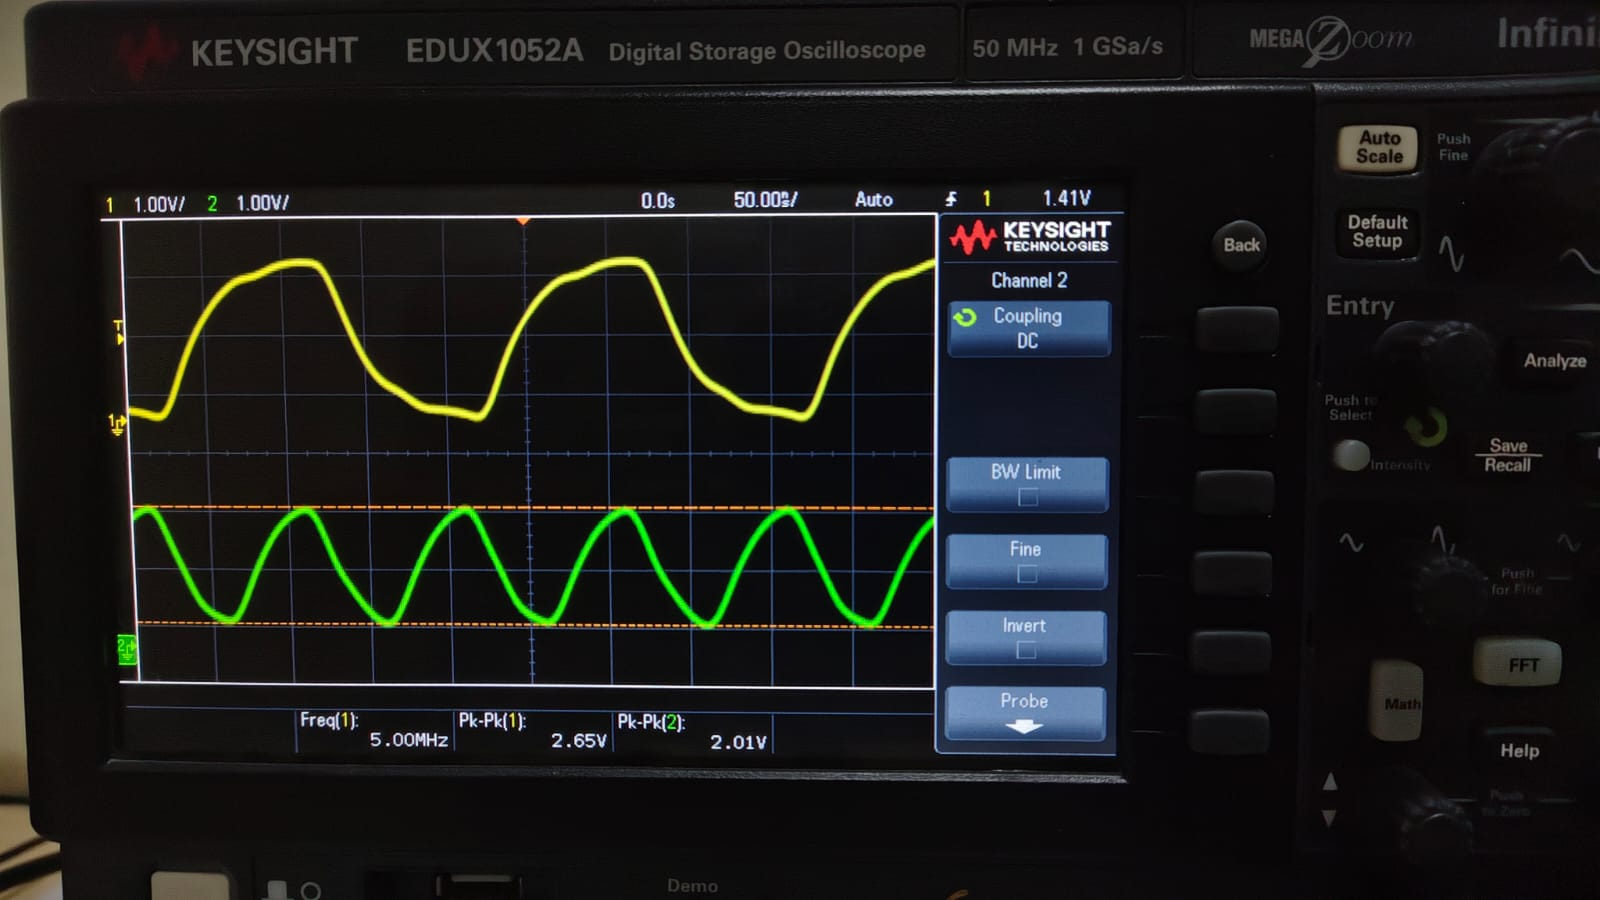
\includegraphics[width=\linewidth]{../images/10Mclk-whoami.jpeg}
      \vspace{0.1cm}
      \tiny \textbf{10 MHz Clock Capture:} \texttt{WHO\_AM\_I} transaction shifting out \texttt{SENSOR\_ID = 8'd9} on MISO.
    \end{column}
    \begin{column}{0.5\textwidth}
      \centering
      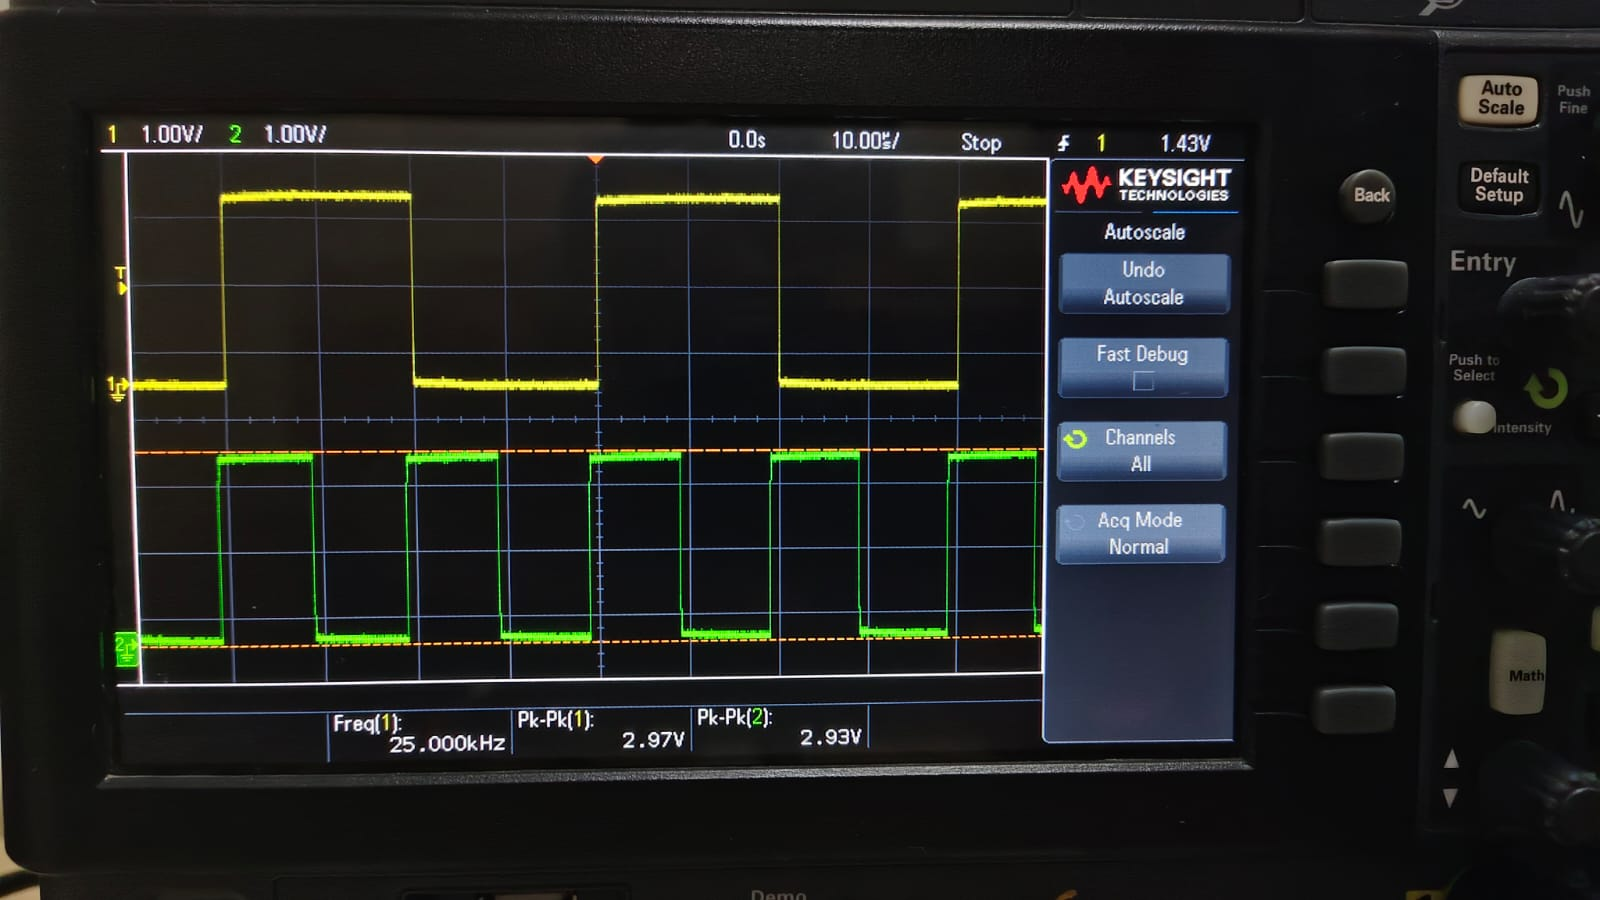
\includegraphics[width=\linewidth]{../images/50khz_clk-whoami.jpeg}
      \vspace{0.1cm}
      \tiny \textbf{50 kHz Clock Capture:} Verification of low-speed clock stability with zero bit loss.
    \end{column}
  \end{columns}
  \vspace{0.2cm}
  \scriptsize
  \textbf{Result:} Opcode \texttt{2'b11} correctly triggers \texttt{WHO\_AM\_I\_STATE}, reliably streaming out the 8-bit identifier across wide frequency ranges ($50\text{ kHz}$ to $10\text{ MHz}$).
\end{frame}

% Slide 18: Sensor Read Capture
\begin{frame}{Hardware Sensor Data Read Capture}
  \centering
  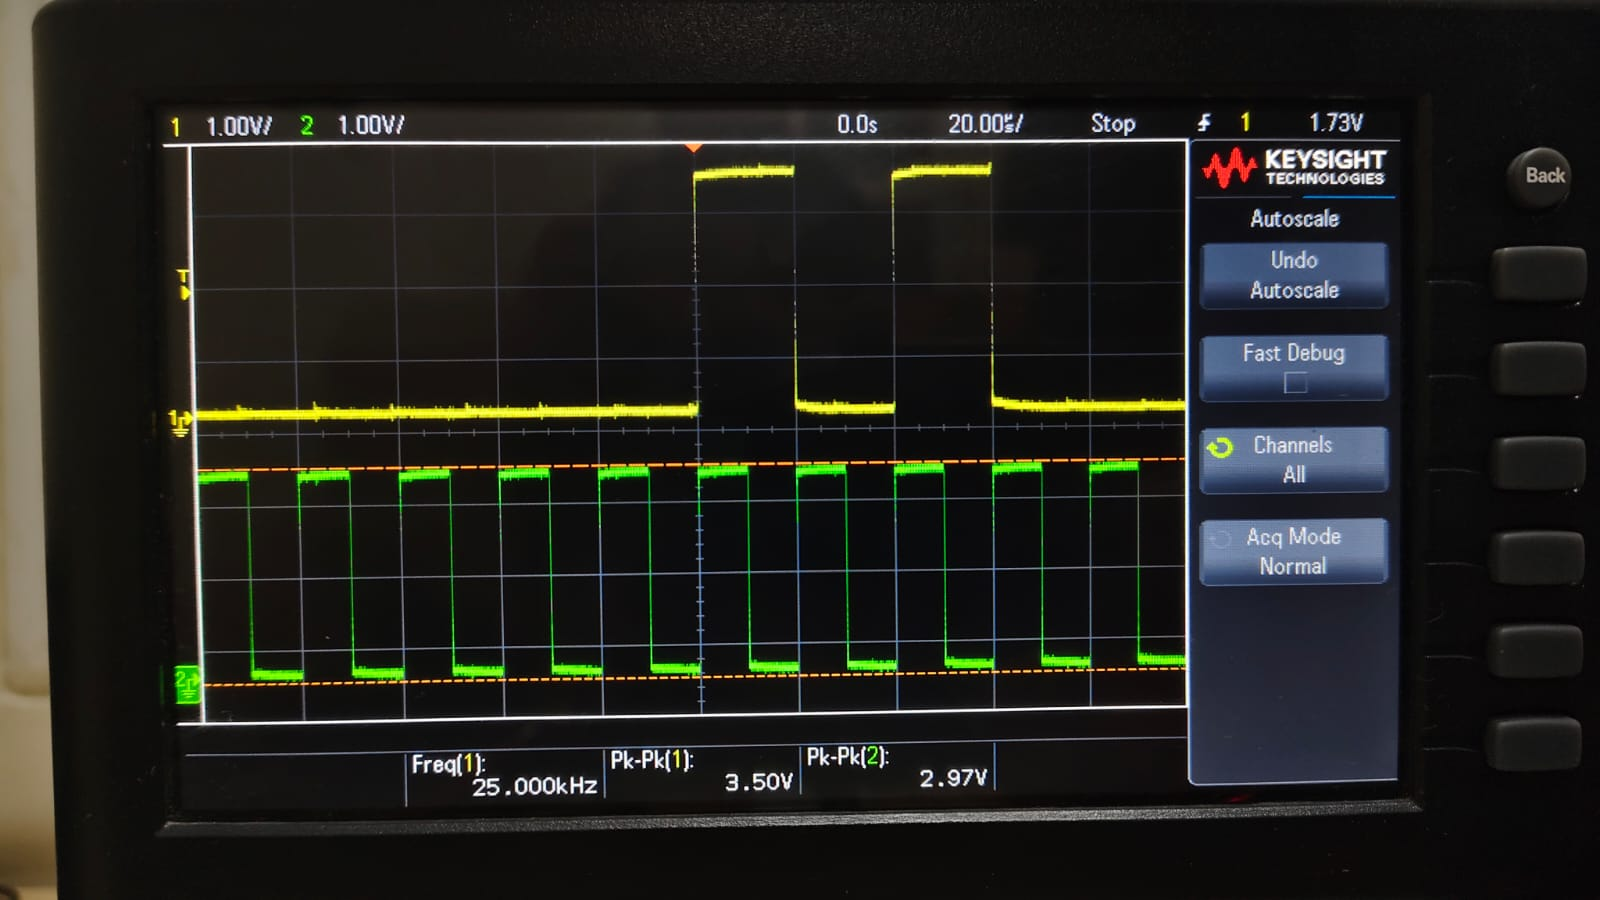
\includegraphics[width=0.85\linewidth]{../images/50khz_clk_read_sensor_A.jpeg}
  \vspace{0.15cm}
  \begin{itemize}
    \scriptsize
    \item Logic analyzer trace of Sensor Read operation at $50\text{ kHz}$ SCLK.
    \item Verifies parallel data transfer from physical DIP switches to serial stream on MISO.
  \end{itemize}
\end{frame}

% Slide 19: Read MOSI/MISO Oscilloscope Captures
\begin{frame}{MOSI Read Command \& MISO Response Signals}
  \begin{columns}
    \begin{column}{0.5\textwidth}
      \centering
      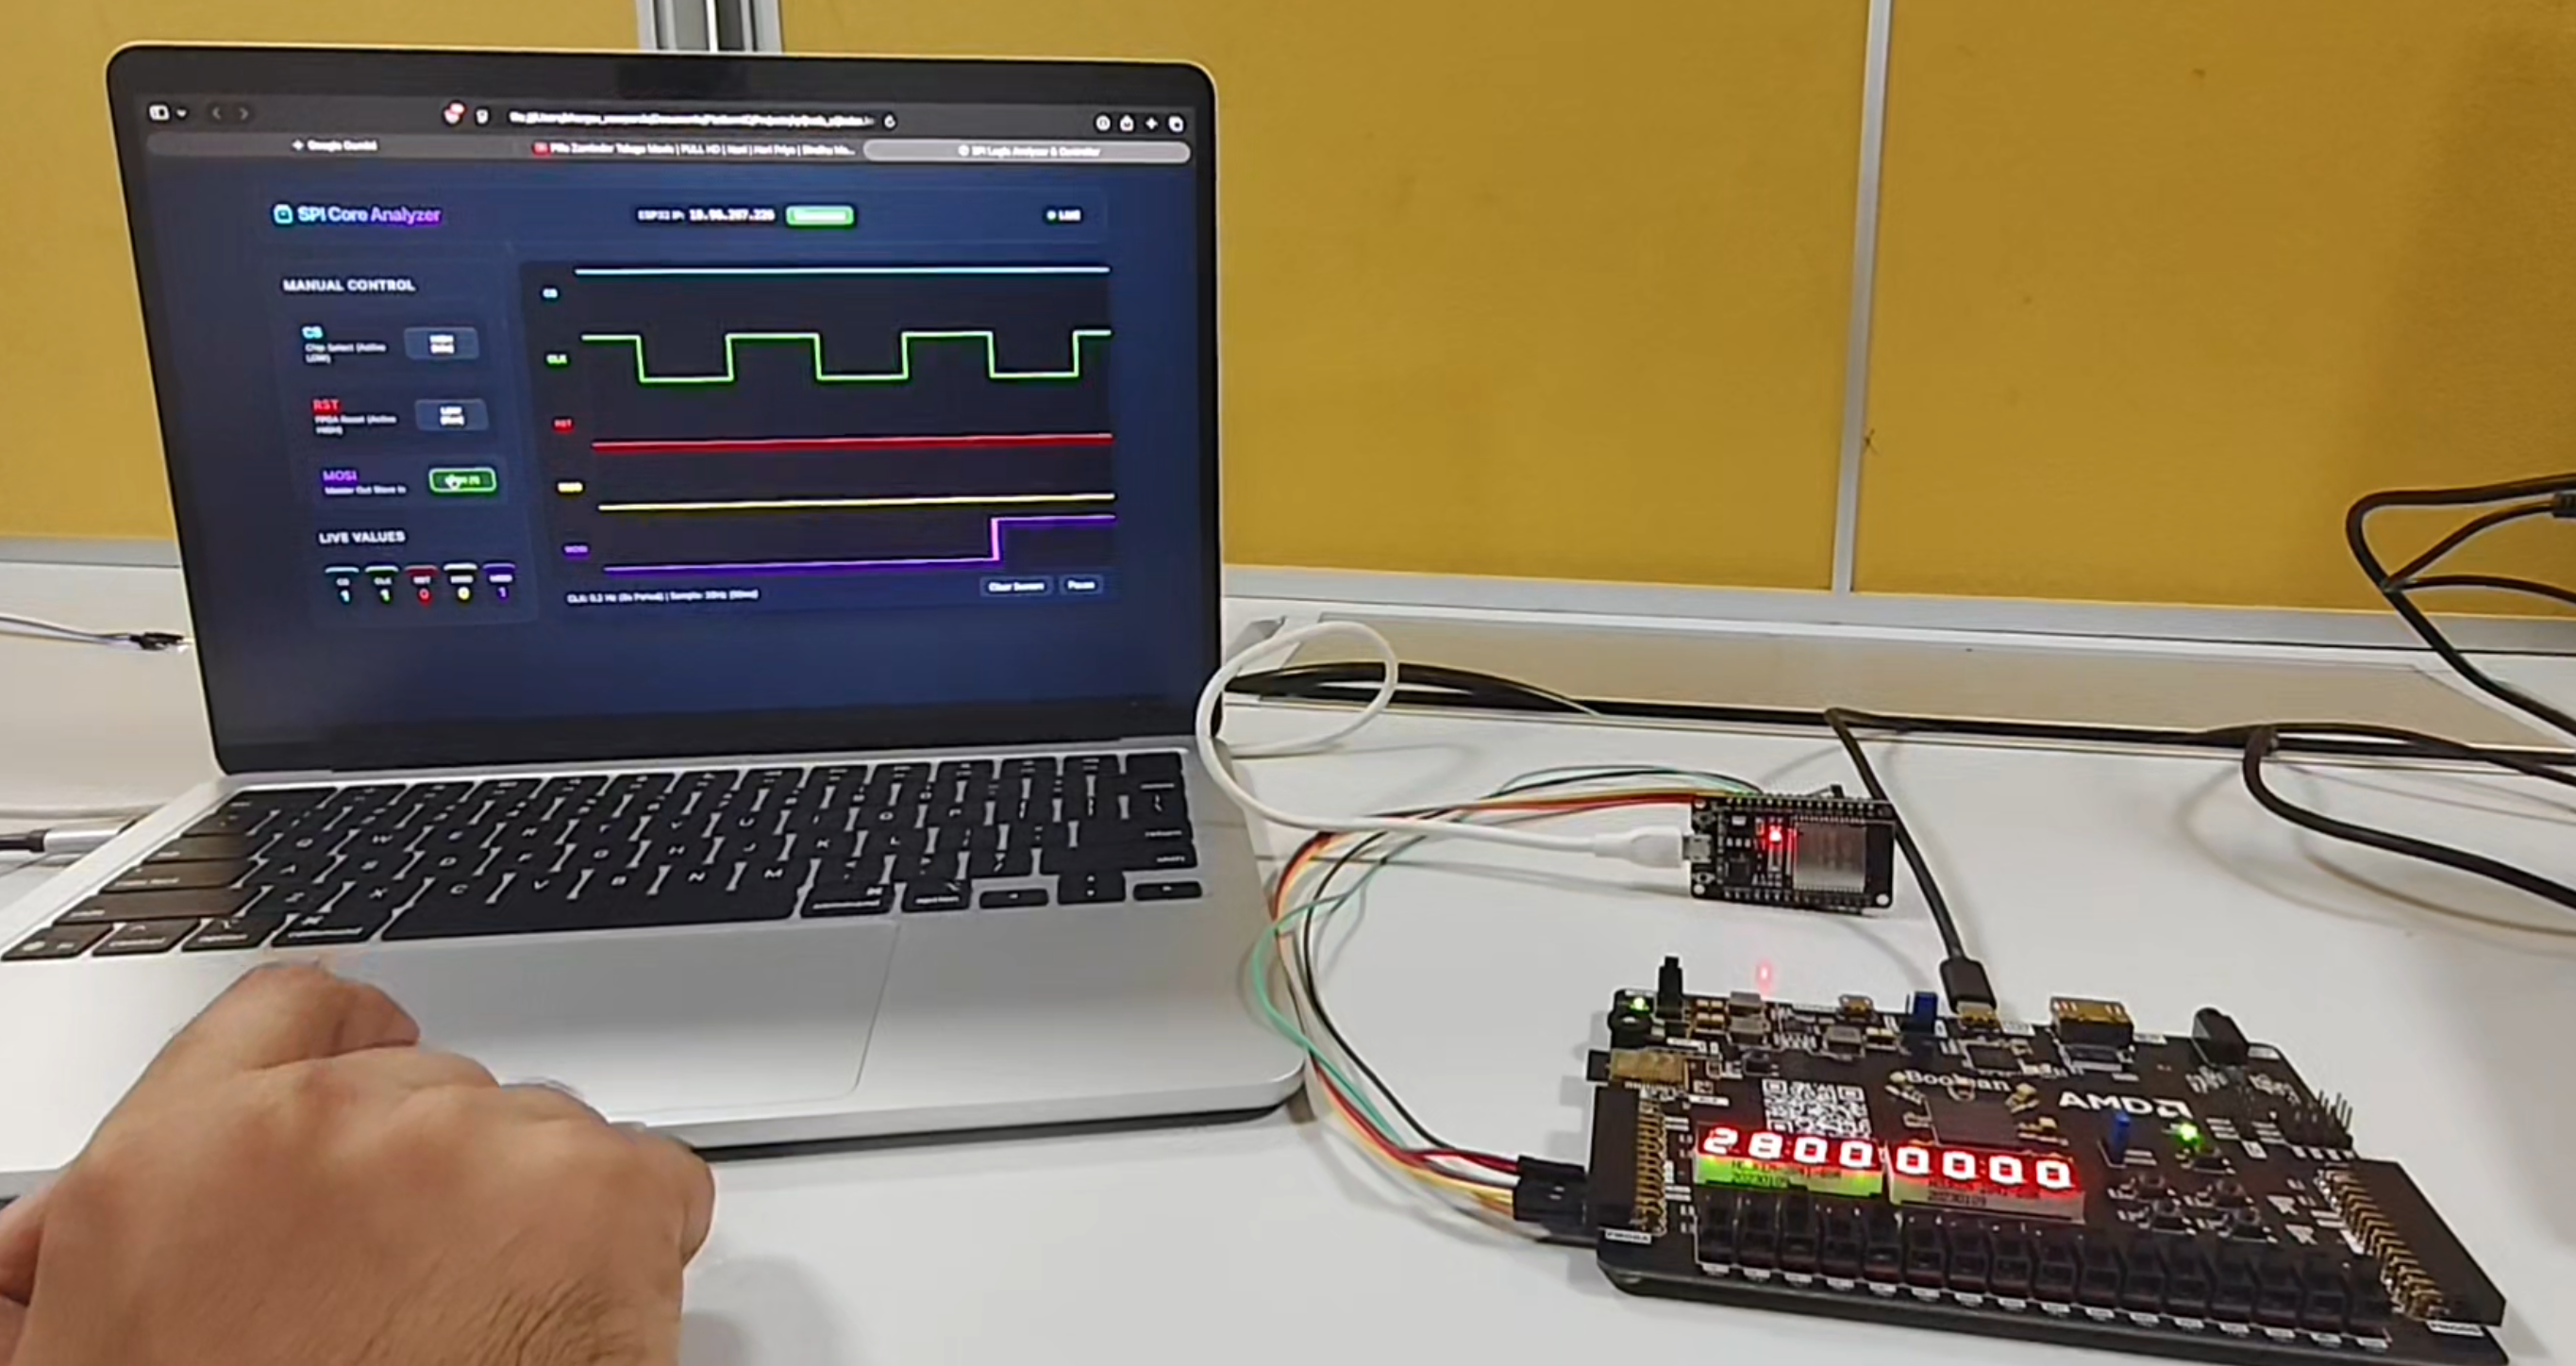
\includegraphics[width=\linewidth]{../images/asking_read_MOSI.png}
      \vspace{0.1cm}
      \tiny \textbf{(a) MOSI Read Command:} Master transmitting opcode \texttt{00} and address frame.
    \end{column}
    \begin{column}{0.5\textwidth}
      \centering
      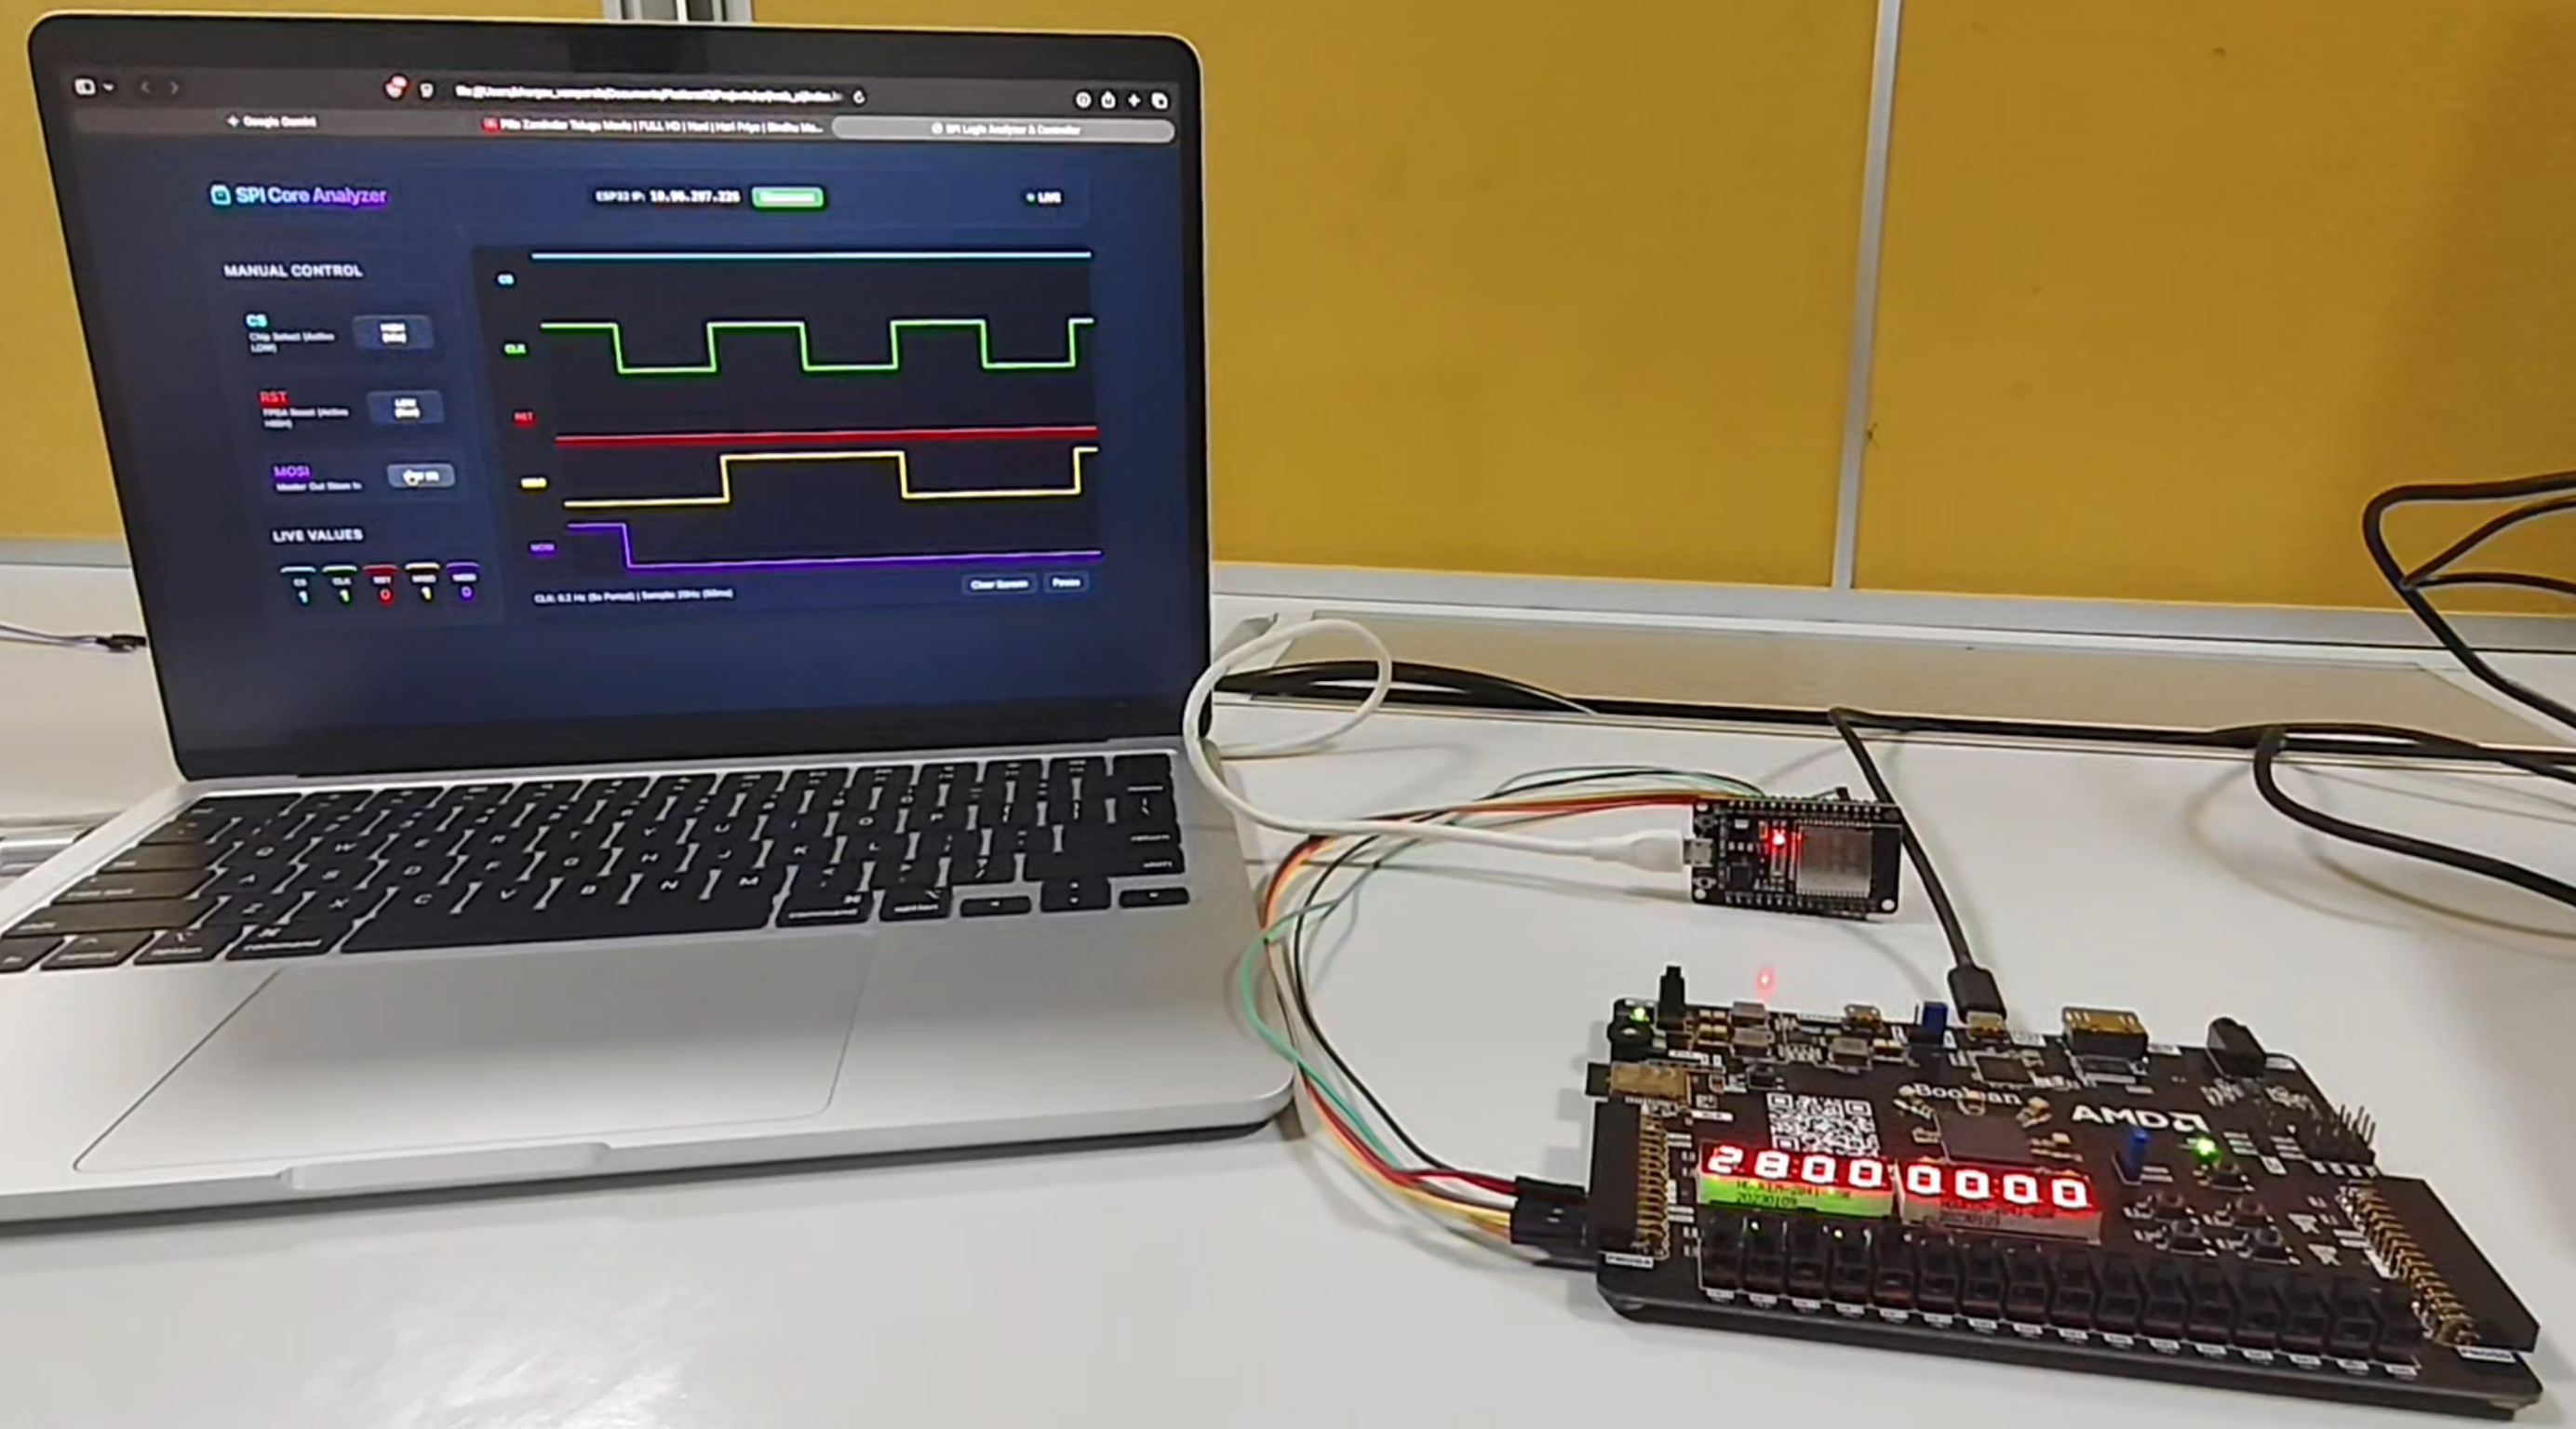
\includegraphics[width=\linewidth]{../images/reciving_read_MISO.png}
      \vspace{0.1cm}
      \tiny \textbf{(b) MISO Read Response:} FPGA streaming register data back to host master.
    \end{column}
  \end{columns}
\end{frame}

% Slide 20: Write Signal Captures
\begin{frame}{Write Transaction Oscilloscope Signals}
  \begin{columns}
    \begin{column}{0.5\textwidth}
      \centering
      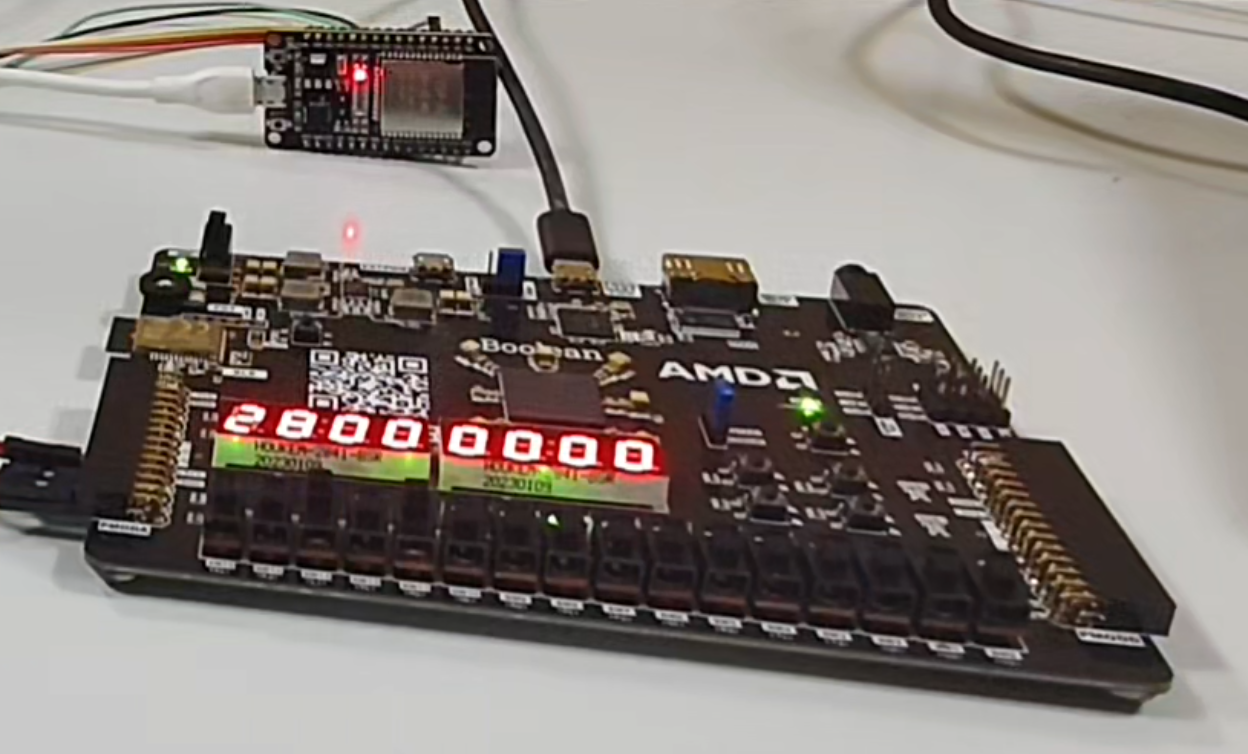
\includegraphics[width=\linewidth]{../images/write-1.png}
      \vspace{0.1cm}
      \tiny \textbf{(a) Write Sequence Start:} Opcode \texttt{01} and address decoding phase.
    \end{column}
    \begin{column}{0.5\textwidth}
      \centering
      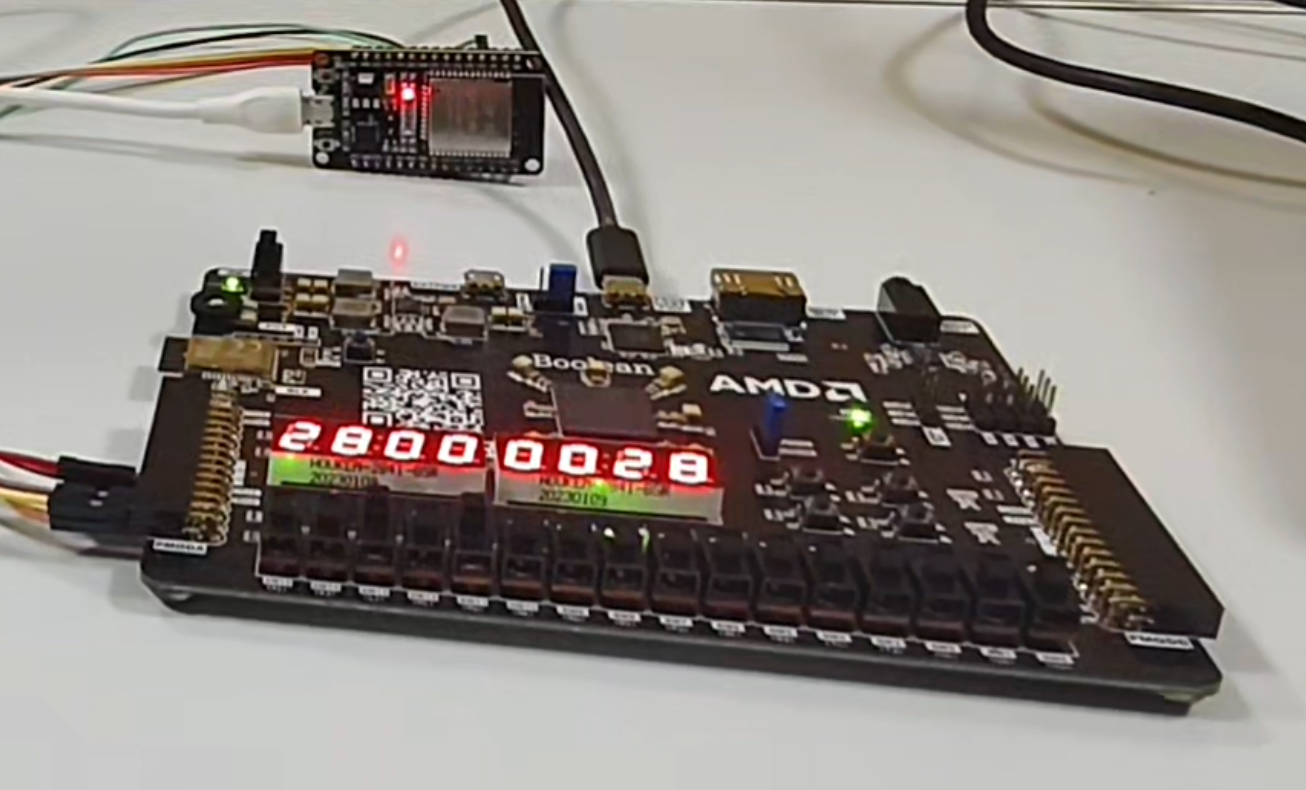
\includegraphics[width=\linewidth]{../images/write-2.png}
      \vspace{0.1cm}
      \tiny \textbf{(b) Write Payload Transfer:} Data bits shifting into \texttt{write\_reg}.
    \end{column}
  \end{columns}
\end{frame}

\section{Simulation \& Case Studies}

% Slide 21: Case Study 1
\begin{frame}{Case Study 1: Sensor Data Read (\texttt{0x2800})}
  \begin{columns}
    \begin{column}{0.5\textwidth}
      \centering
      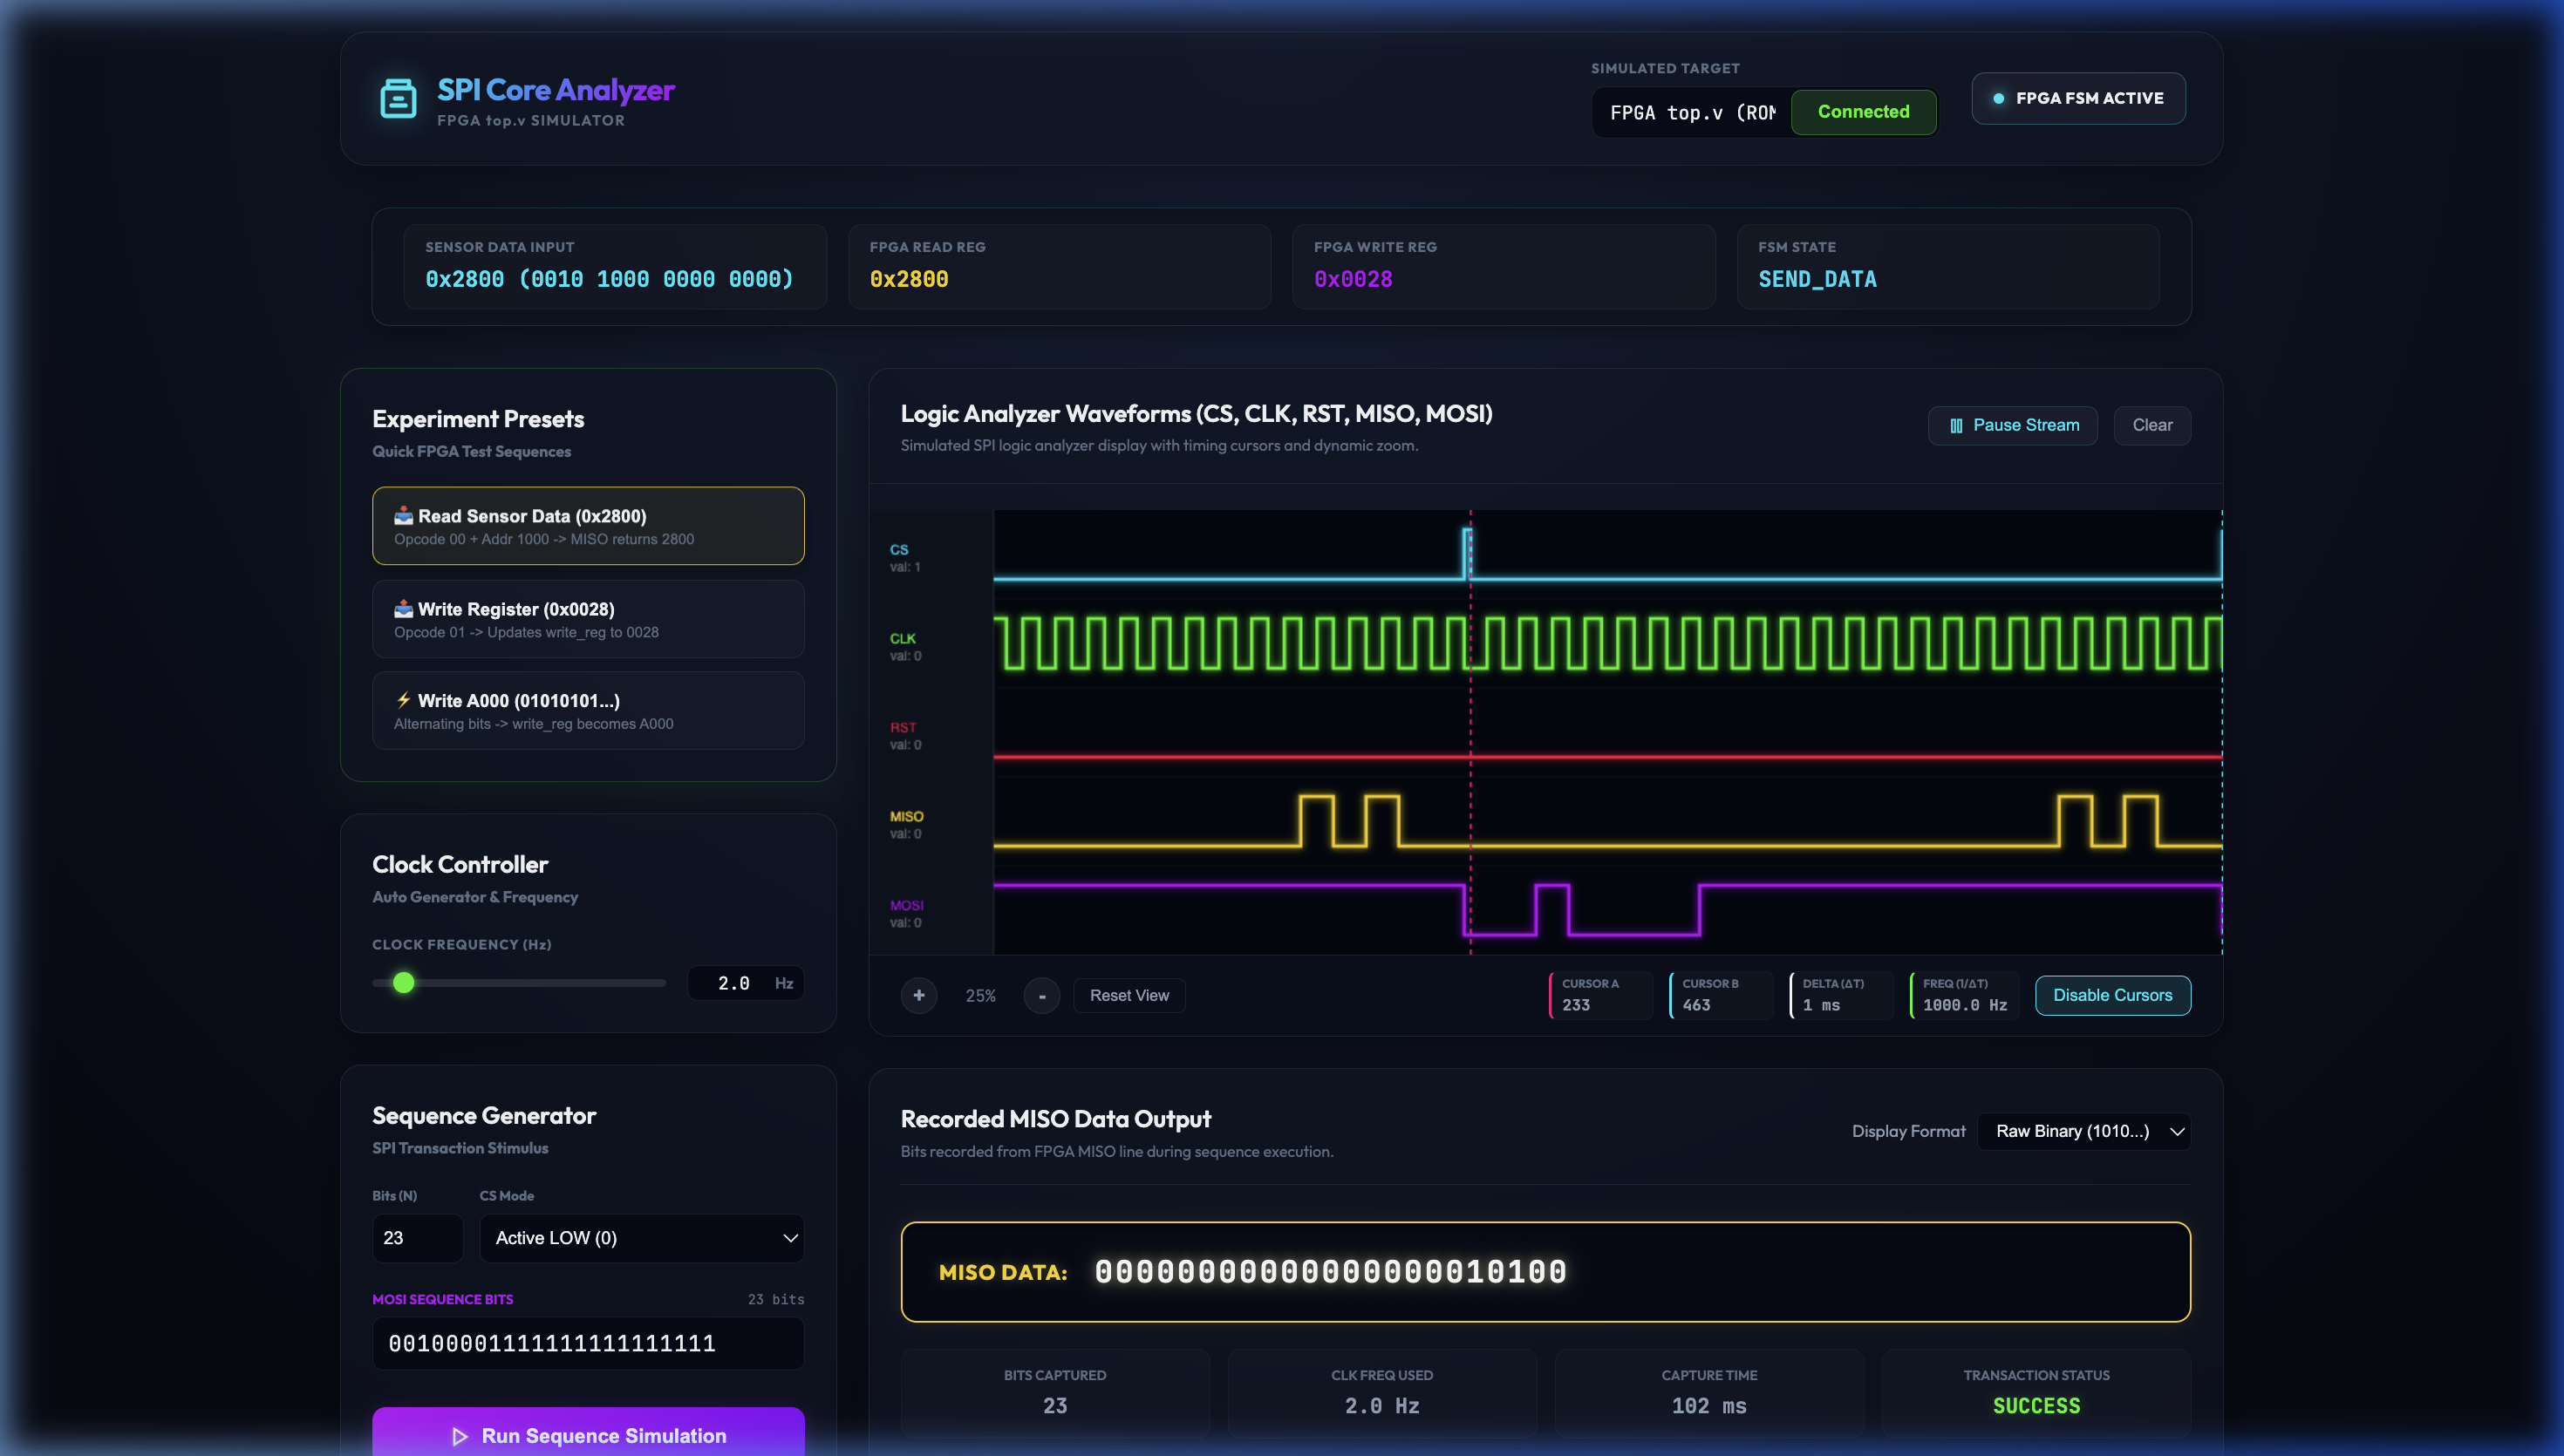
\includegraphics[width=\linewidth]{../images/sim_read_2800.png}
      \vspace{0.1cm}
      \tiny MISO output records \texttt{0010100000000000} (\texttt{0x2800}).
    \end{column}
    \begin{column}{0.5\textwidth}
      \begin{table}
        \centering\tiny
        \begin{tabular}{cclc}
          \toprule
          \textbf{Cycle} & \textbf{MOSI} & \textbf{FSM State} & \textbf{MISO Output} \\
          \midrule
          1 & \texttt{0} & \texttt{DETECT} & \texttt{0} \\
          2 & \texttt{0} & \texttt{DETECT} (Op \texttt{00}) & \texttt{0} \\
          3..6 & \texttt{1000} & \texttt{READ\_ADDR} & \texttt{0} \\
          7 & \texttt{0} & \texttt{SEND\_DATA} & \texttt{0} \\
          8 & \texttt{0} & \texttt{SEND\_DATA} & \texttt{0} \\
          9 & \texttt{0} & \texttt{SEND\_DATA} & \textbf{\texttt{1}} \\
          10 & \texttt{0} & \texttt{SEND\_DATA} & \texttt{0} \\
          11 & \texttt{0} & \texttt{SEND\_DATA} & \textbf{\texttt{1}} \\
          12..22 & \texttt{0...} & \texttt{SEND\_DATA} & \texttt{0} \\
          \bottomrule
        \end{tabular}
      \end{table}
    \end{column}
  \end{columns}
\end{frame}

% Slide 22: Case Study 2
\begin{frame}{Case Study 2: Register Write (\texttt{0x0028})}
  \begin{columns}
    \begin{column}{0.5\textwidth}
      \centering
      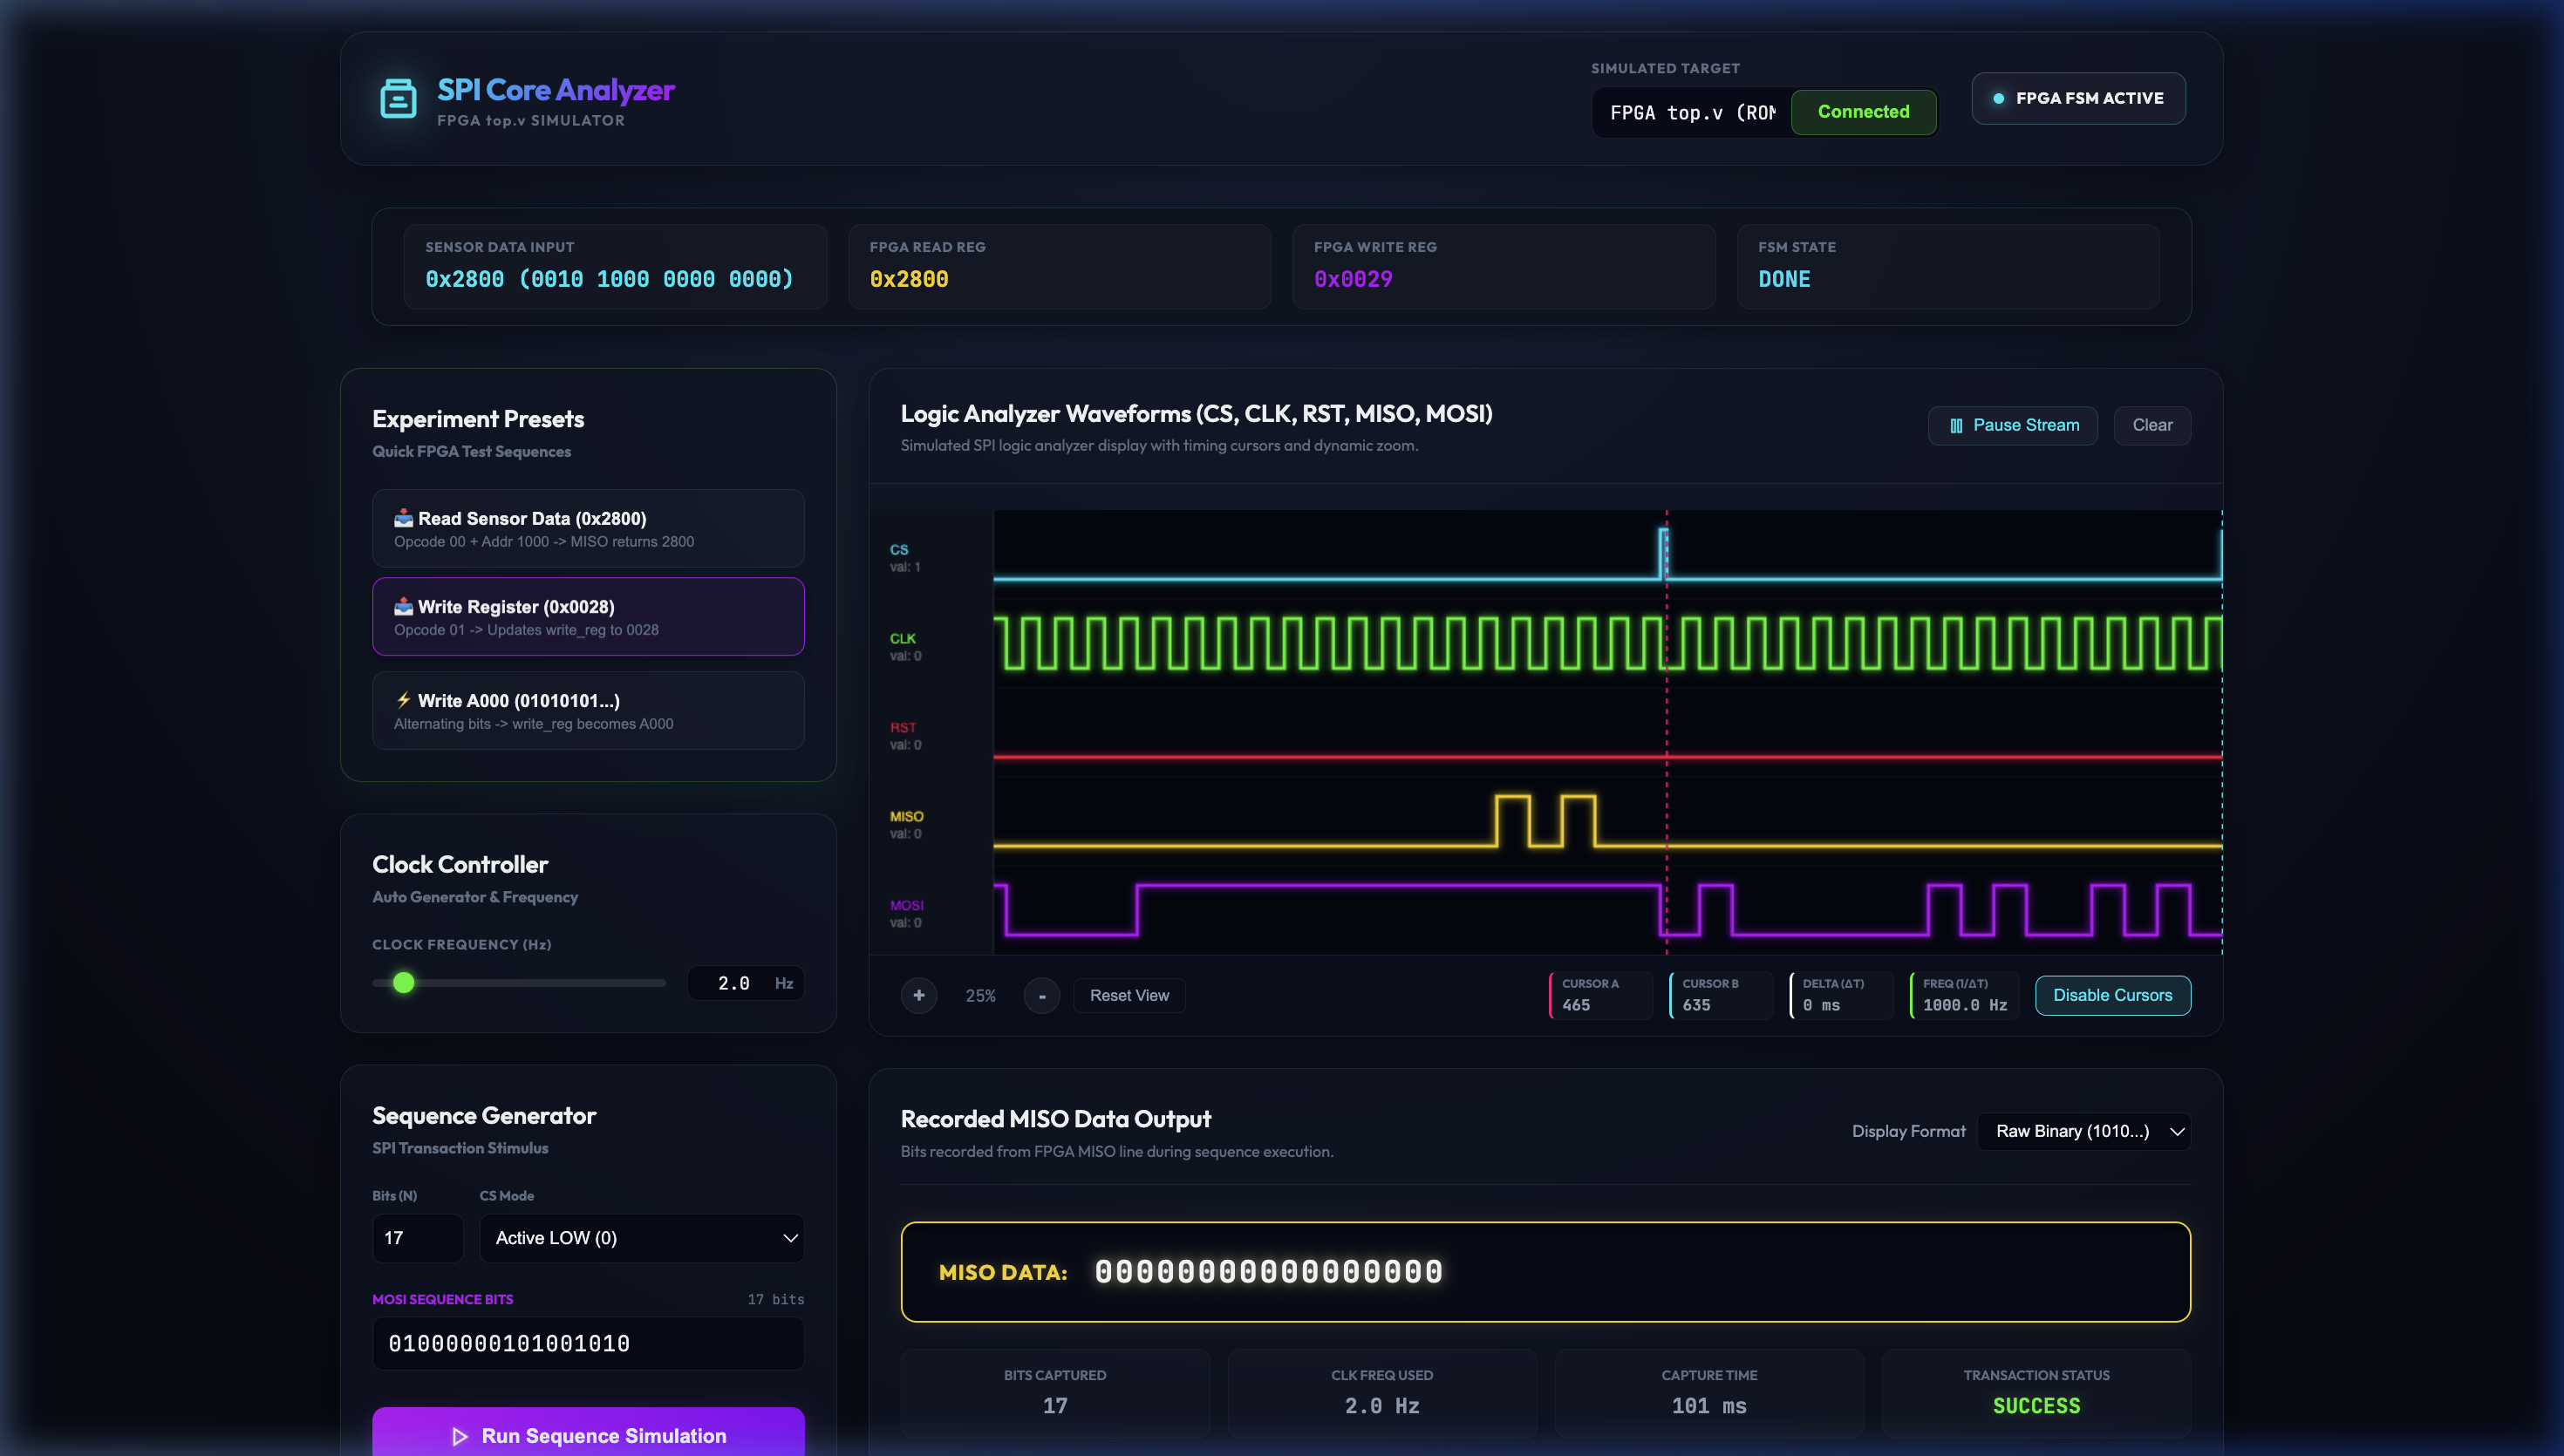
\includegraphics[width=\linewidth]{../images/sim_write_0028.png}
      \vspace{0.1cm}
      \tiny \texttt{write\_reg} successfully updated to \texttt{0x0028}.
    \end{column}
    \begin{column}{0.5\textwidth}
      \begin{table}
        \centering\tiny
        \begin{tabular}{cclc}
          \toprule
          \textbf{Cycle} & \textbf{MOSI} & \textbf{FSM State} & \textbf{write\_reg} \\
          \midrule
          1..2 & \texttt{01} & \texttt{DETECT} (Write) & \texttt{0x0000} \\
          3..6 & \texttt{0000} & \texttt{WRITE\_ADDR} & \texttt{0x0000} \\
          7..10 & \texttt{0101} & \texttt{WRITE\_LEN} (6b) & \texttt{0x0000} \\
          11..13 & \texttt{000} & \texttt{WRITE\_DATA} & \texttt{0x0000} \\
          14 & \texttt{1} & \texttt{WRITE\_DATA} (Bit 3) & \texttt{0x0008} \\
          15 & \texttt{0} & \texttt{WRITE\_DATA} & \texttt{0x0008} \\
          16 & \texttt{1} & \texttt{WRITE\_DATA} (Bit 5) & \textbf{\texttt{0x0028}} \\
          \bottomrule
        \end{tabular}
      \end{table}
    \end{column}
  \end{columns}
\end{frame}

% Slide 23: Case Study 3: 010101 Phenomenon
\begin{frame}{Case Study 3: The \texttt{010101...} Phenomenon (\texttt{0xA000})}
  \begin{itemize}
    \item \textbf{Observed Phenomenon:} Sending alternating bit sequence \texttt{0101010101...} turned \texttt{write\_reg} from \texttt{0000} to \texttt{A000}.
  \end{itemize}
  \begin{columns}
    \begin{column}{0.4\textwidth}
      \centering
      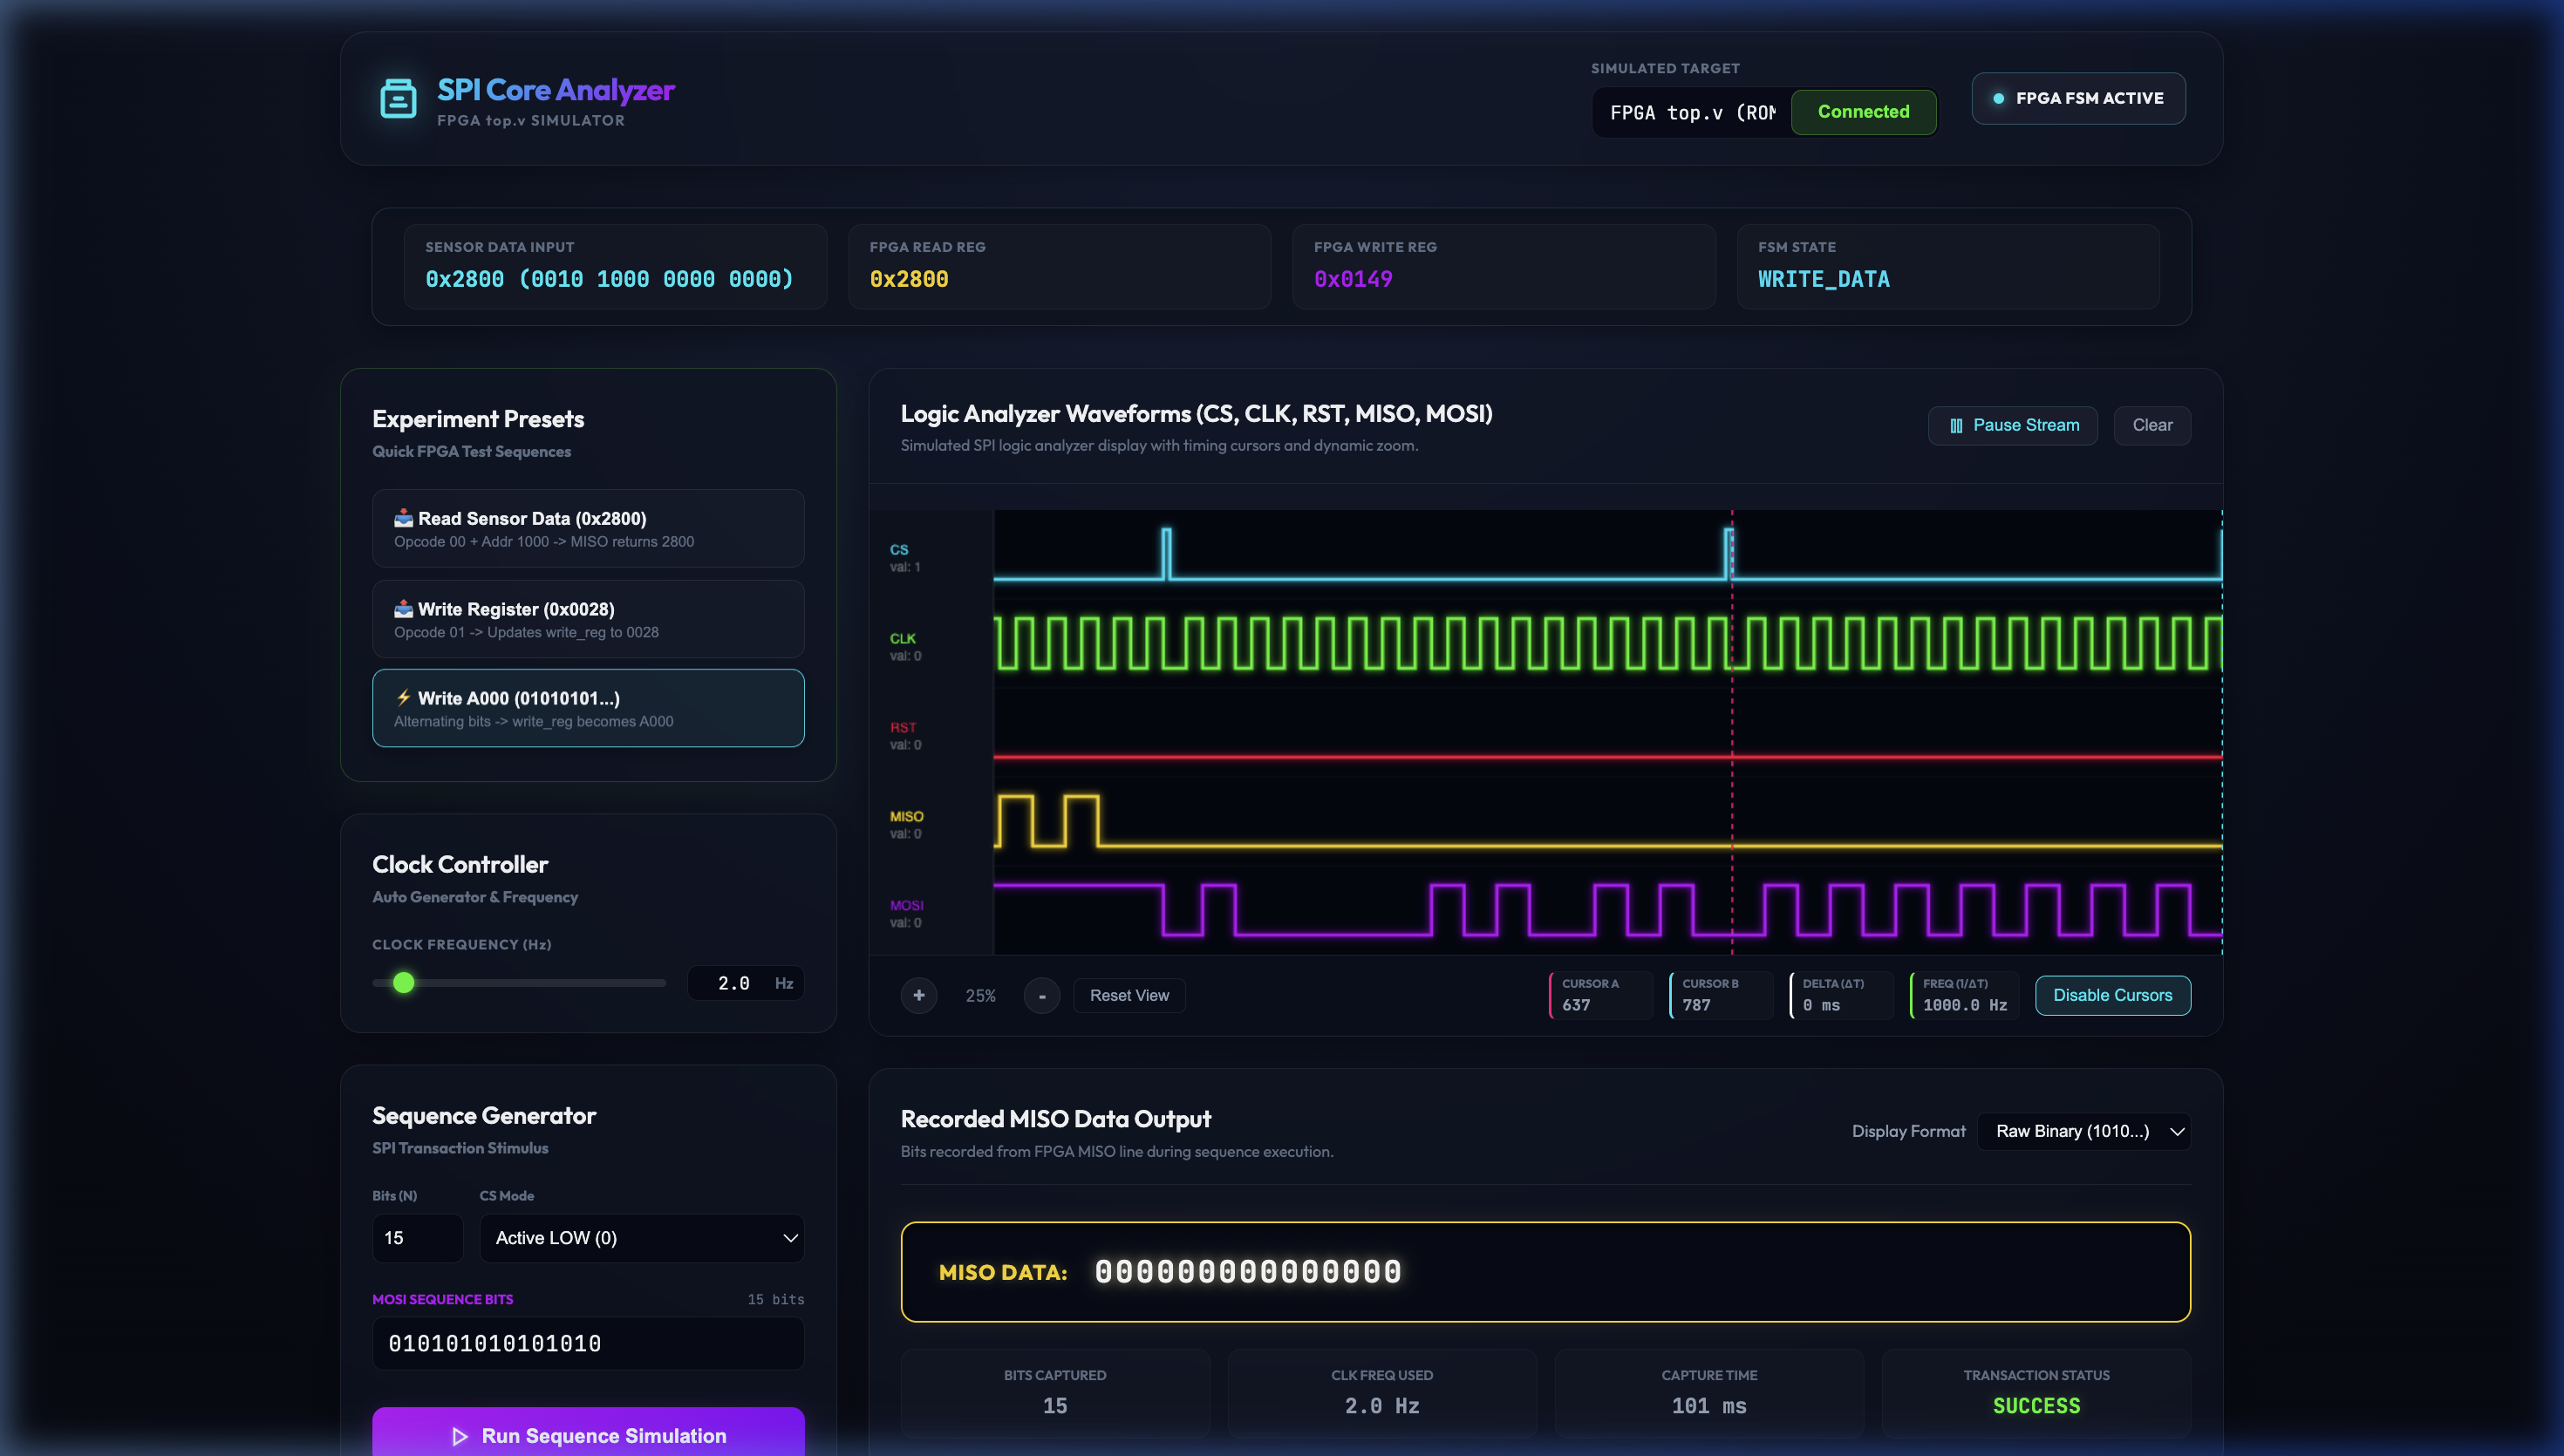
\includegraphics[width=\linewidth]{../images/sim_write_a000.png}
      \vspace{0.05cm}
      \tiny Web simulation capture.
    \end{column}
    \begin{column}{0.3\textwidth}
      \centering
      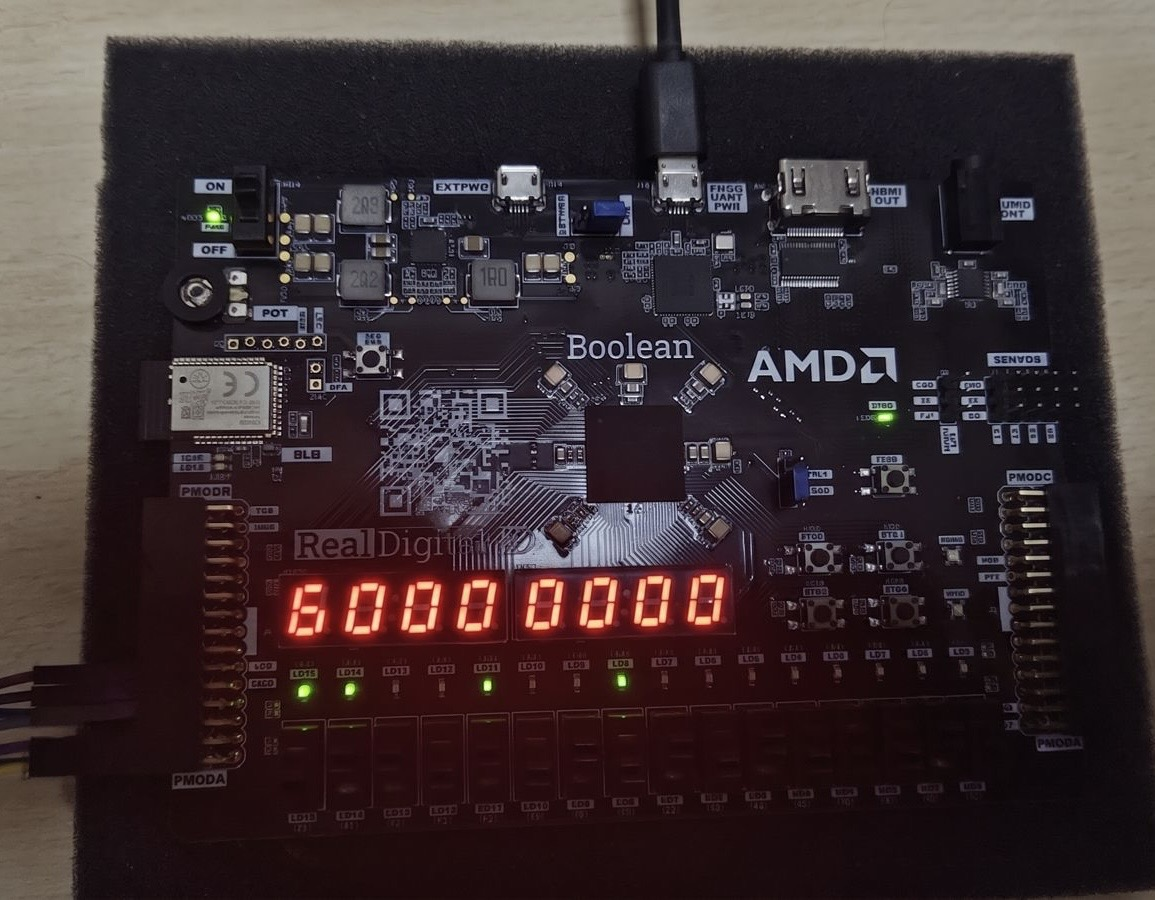
\includegraphics[width=\linewidth]{../images/0000.jpg}
      \vspace{0.05cm}
      \tiny Initial state (\texttt{0000}).
    \end{column}
    \begin{column}{0.3\textwidth}
      \centering
      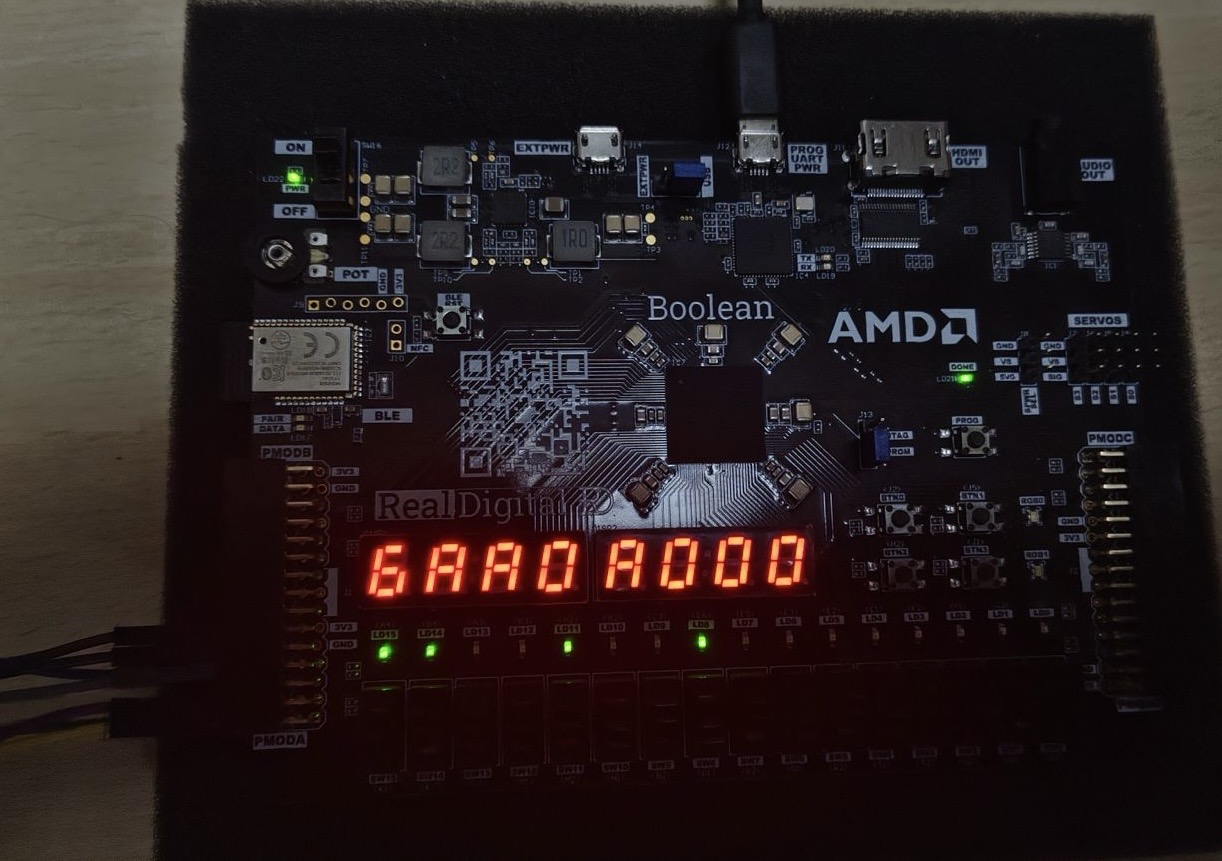
\includegraphics[width=\linewidth]{../images/A000.jpg}
      \vspace{0.05cm}
      \tiny Final state (\texttt{A000}).
    \end{column}
  \end{columns}
\end{frame}

% Slide 24: Phenomenon Breakdown
\begin{frame}{Case Study 3: Step-by-Step Bit Parsing Breakdown}
  \begin{enumerate}
    \scriptsize
    \item \textbf{Opcode Decoding (\texttt{DETECT}):}
    \begin{itemize}
      \item Bit 1: \texttt{0}, Bit 2: \texttt{1} $\rightarrow$ Opcode \texttt{2'b01} (Write Command).
    \end{itemize}
    \item \textbf{Address Decoding (\texttt{WRITE\_ADDR}):}
    \begin{itemize}
      \item Bits 3--6: \texttt{0}, \texttt{1}, \texttt{0}, \texttt{1} $\rightarrow$ Address \texttt{4'b0101} = \textbf{\texttt{4'd5}} (Sensor 4).
    \end{itemize}
    \item \textbf{ROM Lookup:}
    \begin{itemize}
      \item For \texttt{4'd5}, ROM yields \texttt{in\_width = 4}, \texttt{in\_start = 12}.
    \end{itemize}
    \item \textbf{Payload Writing (\texttt{WRITE\_DATA}):}
    \begin{itemize}
      \item Bits 7--10: \texttt{0}, \texttt{1}, \texttt{0}, \texttt{1} $\rightarrow$ written to bits 12..15 as \texttt{4'b1010} (\texttt{0xA}).
    \end{itemize}
    \item \textbf{Final Register Value:}
    \begin{itemize}
      \item \texttt{16'b1010\_0000\_0000\_0000} $\rightarrow$ \textbf{\texttt{16'hA000}}.
    \end{itemize}
  \end{enumerate}
\end{frame}

\section{Experimental Results}

% Slide 25: Resource Utilization
\begin{frame}{FPGA Resource Utilization \& Timing Analysis}
  \begin{table}
    \centering\small
    \begin{tabular}{lccc}
      \toprule
      \textbf{FPGA Resource} & \textbf{Method 1} & \textbf{Method 2} & \textbf{Available (Artix-7)} \\
      \midrule
      LUTs & 78 & 62 & 20,800 \\
      Flip-Flops & 68 & 54 & 41,600 \\
      BRAM Blocks & 0 & 0 & 50 \\
      Setup Slack & $+15.24\text{ ns}$ & $+15.24\text{ ns}$ & Target: 50 MHz \\
      Max Frequency ($F_{\text{max}}$) & $142.8\text{ MHz}$ & $166.4\text{ MHz}$ & — \\
      \bottomrule
    \end{tabular}
    \caption{Resource and Timing Analysis Report}
  \end{table}
  \begin{itemize}
    \item \textbf{Logic Savings:} Method 2 achieves a \textbf{20.5\% reduction in LUT usage} and a \textbf{20.6\% reduction in FFs} due to a streamlined state machine (6 vs 9 states).
  \end{itemize}
\end{frame}

% Slide 26: Latency & Throughput Comparison
\begin{frame}{Quantitative Protocol Latency \& Throughput}
  \begin{block}{Latency Equations}
    \begin{align*}
      \text{Latency}_{\text{Method 1}} &= T_{\text{detect}} + T_{\text{addr}} + T_{\text{len}} + T_{\text{payload}} = 11 + N \text{ cycles} \\
      \text{Latency}_{\text{Method 2}} &= T_{\text{detect}} + T_{\text{addr}} + T_{\text{payload}} = 6 + N \text{ cycles}
    \end{align*}
  \end{block}
  \begin{itemize}
    \item For a standard 4-bit write transaction ($N=4$):
    \begin{itemize}
      \item \textbf{Method 1:} 15 clock cycles ($1.50\ \mu\text{s}$ at $10\text{ MHz}$).
      \item \textbf{Method 2:} 10 clock cycles ($1.00\ \mu\text{s}$ at $10\text{ MHz}$).
      \item \textbf{Speedup:} \textbf{33.3\% reduction in transaction latency}.
    \end{itemize}
    \item \textbf{Continuous Throughput:} Method 2 reaches $7.14\text{ Mbps}$ vs. $5.26\text{ Mbps}$ for Method 1.
  \end{itemize}
\end{frame}

% Slide 27: Pros/Cons Comparison
\begin{frame}{Methodology Tradeoffs \& Selection Guidelines}
  \begin{table}
    \centering\tiny
    \begin{tabular}{lp{4.2cm}p{4.2cm}}
      \toprule
      \textbf{Method} & \textbf{Advantages (Pros)} & \textbf{Drawbacks (Cons)} \\
      \midrule
      \textbf{Method 1: Address + Length} & 
        - Software-defined dynamic widths \newline
        - No re-synthesis needed for new sensors \newline
        - High runtime flexibility & 
        - High control overhead (11 bits/write) \newline
        - Higher transaction latency \newline
        - Larger FSM logic footprint \\
      \midrule
      \textbf{Method 2: ROM Lookup} & 
        - Low control overhead (6 bits/write) \newline
        - 33.3\% faster data transfers \newline
        - 20.5\% smaller FPGA logic footprint & 
        - Hardcoded register metadata \newline
        - Requires FPGA bitstream rebuild to update \newline
        - Constrained by ROM depth \\
      \bottomrule
    \end{tabular}
  \end{table}
\end{frame}

\section{Conclusion \& Future Work}

% Slide 28: Conclusion
\begin{frame}{Conclusion \& Summary of Accomplishments}
  \begin{itemize}
    \item \textbf{Wiring Reduction:} Resolved the $O(N)$ physical wiring problem of traditional multi-slave SPI networks, reducing connections to a constant 3/4-wire bus.
    \item \textbf{CDC FIFO Integration:} Robustly decoupled master clock phases from sensor domains using an asynchronous Gray-code FIFO.
    \item \textbf{Methodology Verification:} Proven 33.3\% latency reduction and 20.5\% logic saving using the ROM Lookup Table protocol.
    \item \textbf{Complete Hardware Verification:} Fully validated via oscilloscope signal captures, Vivado synthesis on Artix-7, and an interactive ESP32 web server interface.
  \end{itemize}
\end{frame}

% Slide 29: Future Work
\begin{frame}{Future Work \& System Extensions}
  \begin{itemize}
    \item \textbf{Programmable RAM Configuration Map:} Replace the static ROM with write-programmable RAM, combining Method 1's runtime flexibility with Method 2's low protocol overhead.
    \item \textbf{Direct Memory Access (DMA):} Integrate a DMA controller to burst sensor data directly to system memory without host CPU intervention.
    \item \textbf{Standard SoC Interconnect Wrappers:} Develop AMBA AXI4-Lite or Wishbone bus wrappers for seamless integration into larger SoC platforms.
  \end{itemize}
\end{frame}

% Slide 30: Thank You Slide
\begin{frame}
  \centering
  \Huge \textbf{Thank You!} \\
  \vspace{0.5cm}
  \Large Questions \& Discussion
\end{frame}

\end{document}
